%%%%%%%%%%%%%%%%%%%%%%%%%%%%%%%%%%%%%%%%%%%%%%%%%%%%%%%%%%%%%%%%%%%%%%%%%%%%
% AGUtmpl.tex: this template file is for articles formatted with LaTeX2e,
% Modified March 2013
%
% This template includes commands and instructions
% given in the order necessary to produce a final output that will
% satisfy AGU requirements.
%
% PLEASE DO NOT USE YOUR OWN MACROS
% DO NOT USE \newcommand, \renewcommand, or \def.
%
% FOR FIGURES, DO NOT USE \psfrag or \subfigure.
%
%%%%%%%%%%%%%%%%%%%%%%%%%%%%%%%%%%%%%%%%%%%%%%%%%%%%%%%%%%%%%%%%%%%%%%%%%%%%
%
% All questions should be e-mailed to latex@agu.org.
%
%%%%%%%%%%%%%%%%%%%%%%%%%%%%%%%%%%%%%%%%%%%%%%%%%%%%%%%%%%%%%%%%%%%%%%%%%%%%
%
% Step 1: Set the \documentclass
%
% There are two options for article format: two column (default)
% and draft.
%
% PLEASE USE THE DRAFT OPTION TO SUBMIT YOUR PAPERS.
% The draft option produces double spaced output.
%
% Choose the journal abbreviation for the journal you are
% submitting to:

% jgrga JOURNAL OF GEOPHYSICAL RESEARCH
% gbc   GLOBAL BIOCHEMICAL CYCLES
% grl   GEOPHYSICAL RESEARCH LETTERS
% pal   PALEOCEANOGRAPHY
% ras   RADIO SCIENCE
% rog   REVIEWS OF GEOPHYSICS
% tec   TECTONICS
% wrr   WATER RESOURCES RESEARCH
% gc    GEOCHEMISTRY, GEOPHYSICS, GEOSYSTEMS
% sw    SPACE WEATHER
% ms    JAMES
% ef    EARTH'S FUTURE
%
%
%
% (If you are submitting to a journal other than jgrga,
% substitute the initials of the journal for "jgrga" below.)

\documentclass[jgrga, draft]{agutex}
% \documentclass[jgrga]{agutex}
% To create numbered lines:

% If you don't already have lineno.sty, you can download it from
% http://www.ctan.org/tex-archive/macros/latex/contrib/ednotes/
% (or search the internet for lineno.sty ctan), available at TeX Archive Network (CTAN).
% Take care that you always use the latest version.

% To activate the commands, uncomment \usepackage{lineno}
% and \linenumbers*[1]command, below:

\usepackage{lineno}
\linenumbers*[1]

%  To add line numbers to lines with equations:
%  \begin{linenomath*}
%  \begin{equation}
%  \end{equation}
%  \end{linenomath*}
\usepackage{amsmath}

\usepackage{enumitem}
%%%%%%%%%%%%%%%%%%%%%%%%%%%%%%%%%%%%%%%%%%%%%%%%%%%%%%%%%%%%%%%%%%%%%%%%%
% Figures and Tables
%
%
% DO NOT USE \psfrag or \subfigure commands.
%
%  Figures and tables should be placed AT THE END OF THE ARTICLE,
%  after the references.
%
%  Uncomment the following command to include .eps files
 % \usepackage[pdflatex]{graphicx}
 \usepackage{graphicx}
 \DeclareGraphicsExtensions{.pdf, .png, .jpg, .eps}
 \graphicspath{ {./figs/} }

%
%  Uncomment the following command to allow illustrations to print
%   when using Draft:
 \setkeys{Gin}{draft=false}
%
% Substitute one of the following for [dvips] above
% if you are using a different driver program and want to
% proof your illustrations on your machine:
%
% [xdvi], [dvipdf], [dvipsone], [dviwindo], [emtex], [dviwin],
% [pctexps],  [pctexwin],  [pctexhp],  [pctex32], [truetex], [tcidvi],
% [oztex], [textures]
%
% See how to enter figures and tables at the end of the article, after
% references.
%
%% ------------------------------------------------------------------------ %%
%
%  ENTER PREAMBLE
%
%% ------------------------------------------------------------------------ %%

% Author names in capital letters:
\authorrunninghead{HAMMAN ET AL.}

% Shorter version of title entered in capital letters:
\titlerunninghead{COASTAL STREAMFLOW FLUX IN RASM}

%Corresponding author mailing address and e-mail address:
\authoraddr{Corresponding author: Bart Nijssen,
Department of Civil \& Environmental Engineering, Box 352700,
University of Washington, Seattle, WA 98195-2700, USA.
(nijssen@uw.edu)}

\begin{document}

%% ------------------------------------------------------------------------ %%
%
%  TITLE
%
%% ------------------------------------------------------------------------ %%


\title{The Coastal Streamflow Flux in the Regional Arctic System Model}

%% ------------------------------------------------------------------------ %%
%
%  AUTHORS AND AFFILIATIONS
%
%% ------------------------------------------------------------------------ %%


% Use \author{\altaffilmark{}} and \altaffiltext{}

% \altaffilmark will produce footnote;
% matching \altaffiltext will appear at bottom of page.

\authors{Joseph Hamman\altaffilmark{1},
Bart Nijssen\altaffilmark{1},
Andrew Roberts\altaffilmark{2},
Anthony Craig\altaffilmark{2},
Wieslaw Maslowski\altaffilmark{2},
and Robert Osinski\altaffilmark{3}}

\altaffiltext{1}{Department of Civil \& Environmental Engineering,
University of Washington, Seattle, WA, USA.}
\altaffiltext{2}{Department of Oceanography, Naval Postgraduate School,
Monterey, CA, USA.}
\altaffiltext{3}{Polish Institute of Oceanology, Sopot, Poland.}


%% ------------------------------------------------------------------------ %%
%
%  ABSTRACT
%
%% ------------------------------------------------------------------------ %%

% >> Do NOT include any \begin...\end commands within
% >> the body of the abstract.

\begin{abstract}
TODO:
% The purpose of the abstract is twofold: (1) state the nature of the investigation and (2) summarize the important conclusions of this investigation. The abstract should be suitable for separate publication in an abstract journal and be adequate for indexing. Make sure to check for the following:
%
% It is set as a single paragraph.
% It is limited to 250 words for all journals except GRL where the limit is 150 words.
% It does not include table or figure mentions.
% If it has reference citations that are part of the sentence, they should be in roman type and have parentheses around the year; parenthetical reference citations will be deleted.
% All abbreviations used in the abstract are defined.
\end{abstract}

%% ------------------------------------------------------------------------ %%
%
%  BEGIN ARTICLE
%
%% ------------------------------------------------------------------------ %%

% The body of the article must start with a \begin{article} command
%
% \end{article} must follow the references section, before the figures
%  and tables.

\begin{article}

%% ------------------------------------------------------------------------ %%
%
%  TEXT
%
%% ------------------------------------------------------------------------ %%

\section{Introduction}
\label{sec:intro}
% [High-level introduction to what this paper is about.]
% BN: I am more used to seeing a paragraph like this at the end of the introduction rather than at the beginning. It is probably just a matter of what I am used to rather than what is better, but it comes over as rather abrupt to me. Leave as is for now, but we may move it down later. (20 years ago we would never use "we" or "I" in a paper, which is clearly also a style element that has changed).
We have implemented the RVIC river routing scheme within the recently developed Regional Arctic System Model (RASM) \citep{Roberts_2015a,Hamman_2016} in order to represent the streamflow flux between the land and ocean model components.
In this paper, we introduce the RVIC streamflow routing model and describe its coupling within RASM.
We evaluate the performance of RVIC in coupled and uncoupled model simulations by comparing model simulated streamflow to in-situ observations.
We also evaluate the coastal streamflow flux relative to other observation and model based datasets commonly used by the Arctic ocean and climate modeling communities.
We compare two RASM simulations, one with coastal runoff and the other without, to highlight the role and importance of accurately representing streamflow in coupled climate simulations in the Arctic region.
A key result of this work is the production of a new spatially-consistent, high-resolution dataset of coastal freshwater fluxes for the Arctic basin and surrounding areas.

% [Overview of the Arctic freshwater budget/cycle and the role of streamflow.]
Approximately 11\% of global terrestrial runoff drains into the Arctic Ocean, which holds only 1.4\% of the Earth's salt water \citep{Lewis_2000,Lammers_2001}.
As a result, the Arctic Ocean has the lowest salinity levels among the Earth's oceans \citep{Steele_2001}.
Streamflow is the largest contributor of freshwater to the Arctic Ocean and comprises approximately 38\% of the total freshwater flux entering the Arctic Ocean; the remainder of which consists of direct precipitation (24\%) over the Arctic Ocean, inflow from the Pacific Ocean (30\%), and inflow from the Atlantic Ocean (8\%).
The streamflow flux to the Arctic Ocean also has a distinct seasonal cycle.
Across the Arctic region, the annual runoff hydrograph is characterized by a prominent spring freshet, with about two-thirds of the annual runoff volume occurring between April and July \citep{Lammers_2001}.
In fact, during the spring and summer months, the fractional contribution of freshwater to the Arctic Ocean from streamflow may be as high as 60\% (uncertainty in this figure is largely driven by the uncertainty in the seasonal cycle of the Bering Straight inflow) \citep{Serreze_2006}.

% [The role of streamflow in ocean/ice dynamics]
Coastal streamflow plays an important role in coastal ocean dynamics and hydrography, as well as in sea ice formation and melt \citep{Weatherly_1996,Rabe_2011,Fichot_2013}.
Runoff from Arctic river basins is the primary source of buoyancy-driven currents such as the Alaska, Siberian, Norwegian, and East Greenland coastal currents \citep[e.g.][]{Morison_2000,Boyd_2002,McGeehan_2012,Myers_2005}.
Coastal currents play important roles in shelf dynamics and shelf-basin interactions, redistributing both fresh water and heat through mixing and entrainment of deeper waters \citep[e.g.][]{Carmack_1989,Rudels_1999,Ekwurzel_2001}.
Buoyancy delivered by rivers also affects the onset of sea ice formation in winter and melt in spring and summer \citep[e.g.][]{Weatherly_1996}.
Water with lower salinity freezes at higher temperatures, and therefore does not have to be cooled as much as higher salinity water to freeze.
Thus, for a warming and freshening Arctic Ocean, the onset of freezing may be partially buffered against regional warming in areas highly influenced by streamflow.
However, the earlier sea ice freeze-up enabled by lower sea surface salinity (SSS) also reduces the amount of heat the upper ocean can lose in the fall, counteracting the impact freshening has on sea ice development \citep{Weatherly_1996,Morison_2012}.
Streamflow is also important for maintaining the stratification of the Arctic Ocean \citep{Nummelin_2015}.
Although warmer water exists at depth in the Arctic Ocean, stratification is maintained by the density gradient between the cold, fresh, mixed layer above and the more saline halocline and Atlantic water layers below \citep{Serreze_2006}.
These stratifying processes limit the heat flux into the surface mixed layer from below.

% [ocean / sea ice specific studies]
The coastal streamflow flux has also been shown to be an important driver of dynamics in coupled ice-ocean models \citep[e.g.][]{Morison_2012,Lique_2015,Large_2009}.
\citet{Newton_2008} applied observed climatological runoff from nine of the largest rivers within the Arctic basin in the Naval Postgraduate School (NPS) Arctic regional Model (NAME).
Their study used passive Lagrangian flow tracers within their model to track the spatial distribution of runoff.
They found the highest concentrations of river runoff along the Siberian coast and identified that freshwater plumes originating as coastal streamflow entered the central Arctic along topographic boundaries.
However, they went on to conclude that the coarse spatial resolution of their model (18 km) was a limiting factor in the interpretation of their results and that future studies evaluating the interaction of streamflow in the Arctic would benefit from higher spatial resolution and improved forcing datasets.
Despite our understanding of the importance of river runoff in Arctic Ocean dynamics, \citet{Nummelin_2015} show that global climate models (GCMs) poorly represent the vertical structure of the Arctic Ocean, with many models failing to accurately reproduce the observed profiles of temperature and salinity in the upper 500 m of the central Arctic Ocean.
They conclude that an accurate representation of the streamflow flux is a key step toward improving the performance of the ocean model components in these models.

The Coordinated Ocean-ice Reference Experiments (CORE) Corrected Inter-Annual Forcing (CIAF) Version 2.0, hereafter referred to as $CORE.v2$, is a widely used ocean model forcing dataset that includes coastal streamflow estimates based on the dataset of \citet{Dai_2009}.
A strength of the $CORE.v2$ dataset is that it provides observed monthly mean streamflow on a global 1$^{\circ}$ x 1$^{\circ}$ grid, blended with model results to fill temporal gaps and to provide streamflow estimates in ungauged areas.
This blending approach may also be viewed as a weakness of the dataset as it introduces spatial and temporal discontinuities when observations are unavailable.
As we will show in Section \ref{sec:results}, these discontinuities are particularly severe in large ungauged areas such as Greenland and the Canadian Archipelago.

% [streamflow routing and other climate models that include coupled land-ocean dynamics]
Most land surface components in Earth system models (ESMs), including the model used in RASM, do not include neighbor communication and therefore must utilize a separate scheme to transport streamflow across the land surface; this process is referred to as streamflow routing.
There are two fundamental approaches to streamflow routing: cell-to-cell (CTC) and source-to-sink (STS).
CTC routing models simulate streamflow by parameterizing the mass flux between neighboring grid cells, explicitly tracking the volume of streamflow from each grid cell to grid cell across the land surface.
CTC routing methods, such as the River Transport Model (RTM) \citep{Branstetter_2003} have been applied globally in a number of GCMs, including in the Community Earth System Model (CESM).
Although CTC models may be more physically based than STS models, they have been shown to be difficult to parameterize across a range of spatial scales \citep{Sushama_2004}, limiting their applicability.
STS routing methods do not explicitly track streamflow between grid cells; instead, they parameterize the distribution and travel time of runoff between source and outlet grid points.
STS routing models \citep[e.g.][]{Lohmann_1996,Naden_1992}, akin to the RVIC model used in this study, have also been previously applied in coupled models \citep[e.g.][]{Olivera_2000}.
In previous applications of STS routing models within coupled GCMs \citep[e.g.][]{Olivera_2000}, the streamflow routing has been applied at coarse spatial resolutions (greater than 200 km) and low-frequency coupling (e.g. daily).

% [Modern day streamflow routing]
New approaches to streamflow routing continue to be developed, adding new routing parameterizations and additional process representation.
Examples from the recent literature include MOSART \citep{Li_2013}, CaMa-Flood \citep{Yamazaki_2009,Yamazaki_2014}, and mizuRoute \citep{Clark_2016}.
While a number of routing schemes have been coupled to ESMs \citep[e.g.]{Sushama_2004,Olivera_2000,Li_2013}, they have rarely been specifically evaluated in terms of coupled land-ocean interactions.
Those studies that have coupled streamflow routing with an ocean model have generally not been run at a sufficiently high spatial resolution required to resolve the coastal currents streamflow-shelf-basin exchange processes (e.g. eddies) that are particularly important in the Arctic.
In their recent synthesis of CMIP5 runoff dynamics, \citet{Bring_2015} conclude that a significant community effort should be made to improve the understanding and modeling of basin scale freshwater fluxes in coupled climate modeling.
This argument is further echoed by \citet{Lique_2015} and \citet{Bring_2016} in their recent review papers on the representation of the Arctic hydrologic cycle in present-day hydrologic and climate models.

% [Arctic Hydrology literature]
Numerous observational and modeling studies have explored the seasonal and inter-annual behavior of Arctic runoff.
\citet{Lammers_2001} compiled the R-ArcticNET database, a regional hydrographic record of mean monthly streamflow observations that included over 3,700 streamflow gauges in the Pan-Arctic region.
The collection of observations in R-ArcticNET was later used by \citet{Shiklomanov_2009} in their investigation of increasing river discharge in the largest Eurasian rivers and by \citet{Tan_2011} in their study of changes in spring snowmelt timing.
\citet{Dai_2009} extended a coastal subset of the R-ArcticNET database through 2007 as part of their study estimating the global continental runoff flux.
\citet{Su_2005}, \citet{Adam_2007}, \citet{Slater_2007}, \citet{Adam_2008},and \citet{Dai_2009} all have used uncoupled land surface models (LSMs), in conjunction with routing schemes to simulate streamflow across the pan-Arctic region.
These studies have led to an improved understanding of the terrestrial hydroclimate in the Arctic and how the seasonal streamflow dynamics in the Arctic basin respond to changes in climate and water management activities.

% [Paper overview]
In this paper, we describe the streamflow to ocean coupling in the Regional Arctic System Model.
We introduce the new RVIC streamflow routing model in Section \ref{sec:models}, detailing its coupling within RASM, and its advancements in terms of parameterization of high-resolution streamflow routing.
We describe the model simulations and observed data that we have used in Section \ref{sec:data}.
In Section \ref{sec:results}, we present results from fully-coupled RASM simulations where the land and ocean are coupled via the streamflow flux.
We compare simulated streamflow to observations at gauging locations and explore the role of the terrestrial freshwater flux in the high-resolution, eddy-resolving ice and ocean components within RASM.
Section \ref{sec:discussion} includes a discussion on the role of streamflow in the Arctic climate system and the scientific advances and drawbacks associated using a source-to-sink routing model such as RVIC.
In Section \ref{sec:discussion}, we also describe a new high-resolution coastal streamflow flux dataset for ocean modeling resulting from a fully-coupled RASM simulation.
Finally, in Section \ref{sec:conclusions}, we provide our conclusions and highlight the potential for further research using RASM.

\section{Models}
\label{sec:models}

\subsection{RASM}
\label{sec:rasm}
The Regional Arctic System Model is a fully-coupled, high spatial and temporal resolution regional ESM applied over the pan-Arctic domain (Figure \ref{fig:rasm_domain}).
Principal goals of the modeling project are to better understand the interaction between physical systems in the Arctic drainage basin, to advance understanding of past and present states of Arctic climate, and to improve seasonal to multi-decadal prediction capabilities of key Arctic indicators.
Model components are coupled using the CESM coupled model framework and the CPL7 flux coupler \citep{Craig_2011}.
Below, we provide a brief description of the five component models in RASM version 1.0 (Figure \ref{fig:rasm_coupling_schematic}).
For the purposes of this paper, we are principally concerned with the coastal streamflow flux and its role in the Arctic Ocean system
Therefore, our description below mainly focuses on the streamflow and ocean model components.
The reader will find additional information on the implementation of individual component models in the RASM-specific references cited below.

\begin{itemize}[leftmargin=+.5in]
\item CICE: The Los Alamos Sea Ice model is a physically-based, dynamic sea ice model \citep{Hunke_2010}.
\citet{Roberts_2015a} provide a description of the application of CICE, version 5, within RASM.
\item POP: The Parallel Ocean Program model is a general circulation ocean model \citep{Smith_2010}.
\citet{Maslowski_2012}, \citet{Roberts_2015a}, and \citet{Osinski_2016} provide a descriptions of the application of POP, version 2, within RASM.
Of particular relevance to this study, POP uses a virtual salinity flux ($VSF$) to represent changes in ocean salinity due to surface fluxes of freshwater (runoff, ice melt, precipitation, and evaporation).
The $VSF$ is the equivalent amount of salt that would have to be added or removed from a grid cell to obtain the same change in salinity for a given fresh water flux.
It is calculated as
\begin{equation}
  \label{eq:SaltFlux}
  VSF=-F_w S
\end{equation}

where $F_w$ is the sum of the freshwater fluxes from streamflow, precipitation, evaporation, and sea ice melting and freezing, and $S$ is the reference salinity, which is the surface salinity of the grid cell receiving the freshwater flux.

The POP model was initialized from a no-motion state, with climatological temperature and salinity fields derived from the University of Washington Polar Science Center Hydrographic Climatology version 3.0 \citep{Steele_2001}.
The model 75-year spin up consisted of an initial integration starting from 1948 through 1992 followed by a second integration from 1948 through 1979, both forced with $CORE.v2$ (see Section \ref{sec:data}).

\item VIC: The Variable Infiltration Capacity model \citep{Liang_1994} is a macroscale land surface hydrology model.
\citet{Hamman_2016} provide a description of the application of VIC within RASM.
\item WRF: The Weather Research and Forecasting atmospheric model \citep{Skamarock_2007} is a mesoscale meteorological model.
\citet{Cassano_2016} provide a detailed description of the WRF model, version 3.2, as it is applied in RASM.
\item RVIC: The RVIC streamflow routing model is an adapted version of the \citet{Lohmann_1996} linear, source-to-sink routing model frequently used to route the runoff flux from the VIC model.
A complete description of the RVIC model is provided in Section~\ref{sec:rvic}.
\end{itemize}

In RASM Version 1.0, the land, atmosphere, and runoff components share a 50-km near-equal-area North Pole stereographic grid mesh.
The ocean and sea ice models share a 1/12$^{\circ}$ rotated stereographic grid mesh (Figure \ref{fig:rasm_domain}).
All model components are coupled every 20 minutes.
This coupling configuration is described by \citet{Roberts_2015a}, where the sub-daily coupling frequency is shown to be important in reproducing observed inertial frequencies in the atmosphere-ice-ocean coupling cycle.

\subsection{RVIC}
\label{sec:rvic}

The RVIC streamflow routing model is a modified version of the routing model typically used to post-process VIC model output \citep{Lohmann_1996, Lohmann_1998a}.
The original \citet{Lohmann_1996} model has been used in many offline modeling studies from regional to global spatial scales at horizontal resolutions from 1/16$^{\circ}$ to 2$^{\circ}$ \citep[e.g.][]{Nijssen_1997,Lohmann_1998b,Su_2005,Hamlet_2013}.
RVIC is a source-to-sink routing model that solves a linearized version of the Saint-Venant equations \citep{Fread_1992,Mesa_1986}.
The linearized Saint-Venant equations (see Eq. \ref{eq:St_Venant}) are a one-dimensional model describing unsteady flow in terms of two time-invariant parameters, flow velocity and diffusivity.
The velocity and diffusivity parameters can be estimated from observed streamflow or through numeric optimization.
RVIC uses flow direction rasters (FDRs), typically derived from topographic information \citep[e.g.][]{Wu_2011}, to specify the flow path and distance for each source-sink pair.
The flow along the travel path is parameterized as a linear time-invariant unit impulse response function (IRF) to runoff generated at individual grid cells by the LSM.
The notion of the IRF is often referred to as a unit hydrograph (UH) within the field of hydrology \citep[e.g.][]{Sherman_1932,Nash_1957}.
The application of the RVIC model has two distinct steps, a preprocessing step in which IRFs are developed for each source-to-sink pair (see Sections ~\ref{sec:irfs} and ~\ref{sec:remap}), and a computationally efficient convolution step in which distributed runoff from the LSM is routed to downstream points (see Section~\ref{sec:convolution}).

The RVIC model differs from the original \citet{Lohmann_1996} model in four main ways:

\begin{itemize}[leftmargin=+.5in]
\item RVIC completely separates the development of the IRFs from the flow convolution step,
\item RVIC allows the development of the IRFs to be done on FDR grids that do not match the grid elements used for the LSM (see Section~\ref{sec:irfs}),
\item The RVIC convolution scheme operates in a space-before-time pattern, facilitating direct coupling with distributed LSMs (see Section~\ref{sec:convolution}),
\item RVIC includes numerous infrastructure software improvements, including parallel processing, the ability to store the exact model state, and to read and write netCDF files.
\end{itemize}

The stand-alone version of the RVIC model, complete with documentation and example input data, is available via a publicly accessible source code repository \citep{Hamman_2015}.

\subsubsection{Impulse response function development}
\label{sec:irfs}

A UH describes the streamflow response of an area (e.g. basin or grid cell) to a unit input of runoff $Q^F$ in terms of timing and volume (see Figure \ref{fig:uh_remap_schematic}-C).
The development of the IRF for every source-to-sink pair is a combination of an initial UH describing lumped routing behavior of streamflow within the source grid cell, plus the horizontal travel to the downstream point with the addition of a flow diffusivity parameter.
The horizontal travel path and distance are computed using a flow direction raster \citep[e.g.][]{Wu_2011}.
The Saint-Venant equation is given by

 \begin{equation}
   \label{eq:St_Venant}
   \frac{\partial Q}{\partial t} = D \frac{\partial^2 Q}{\partial x} + C \frac{\partial Q}{\partial x}
 \end{equation}

where $Q$ represents the flow at time $t$ at a downstream point $x$ as a function of the wave velocity $C$ and the diffusivity $D$; both of which may be estimated from geographical data.
Eq.~(\ref{eq:St_Venant}) can be linearized and solved with convolution integrals

 \begin{equation}
   \label{eq:conv_integral}
	  Q(x,t) = \int_0^t UH(t-s)h(x,s)ds
 \end{equation}

where

 \begin{equation}
   \label{eq:Greens_IRF}
	h(x, t) = \frac{x}{2t\sqrt{\pi tD}}exp\left(-\frac{(Ct-x)^2}{4Dt}\right)
 \end{equation}

is a Green's impulse response function, and $UH$ is a unit hydrograph representing the distribution of flow from within each source grid cell to the edge of the source grid cell.
Equations \ref{eq:conv_integral} and \ref{eq:Greens_IRF} are solved to determine the flow response for each source-to-sink pair.

\subsubsection{Upscaling and basin aggregation}
\label{sec:remap}

The original employment of the \citet{Lohmann_1996} model required that the FDR grid and the LSM grid match exactly.
This limited the applicability of the model and required either the LSM to be evaluated on the same grid as an existing flow direction dataset grid or the custom generation of an FDR for each LSM grid.
The RVIC implementation allows the development of the IRFs on an arbitrary grid, usually higher spatial resolution, than the LSM by upscaling and aggregating the high-resolution IRF grid to the LSM grid (Figure \ref{fig:uh_remap_schematic}).
The upscaling process spatially remaps the IRFs from the high-resolution FDR grid to the LSM grid using the first-order conservative remapping technique developed by \citet{Jones_1999}.
Because the remapping scheme is conservative, each of the resulting IRFs on the LSM grid is an area weighted average of the IRFs on the high-resolution FDR grid.
Finally, in the event there are multiple sink points on the FDR grid within a single LSM grid cell, the upscaled IRFs are combined to include all source points flowing into a single outlet grid cell.

\subsubsection{Convolution}
\label{sec:convolution}

The convolution step combines the IRFs with the discharge fluxes from the LSM.
The streamflow $Q$ for each outlet grid cell $x$ and time step $t$ is given by

\begin{equation}
  \label{eq:convolution}
   Q(x,t) = \int_0^{S(x)} \int_0^{\infty}\,IRF(s,t)\,Q^F(s,t-\tau)\,d\tau\,ds
 \end{equation}

where $S(x)$ is the number of source grid cells upstream of each outlet ($x$), and $\tau$ is the position in the IRF vector.
RVIC's application of the convolution is practically equivalent to the one described by \citet{Lohmann_1996}.
The key difference is in the implementation, where the time integral has been moved to the outer loop in RVIC, allowing for stepwise evaluation of the convolution over the entire spatial model domain.

\subsubsection{RVIC in RASM}

The IRFs used in RASM were developed using the 1/16$^{\circ}$ FDRs from \citet{Wu_2011}.
RVIC in RASM uses a spatially constant flow velocity and diffusivity of 0.6 m/s and a 3,000 m$^2$/s, respectively.
These parameters were chosen using the calibration methods described in Section~\ref{sec:parameters}.
Hourly IRFs were developed for each of the 95,001 coastal 1/16$^{\circ}$ grid cells bordering the ocean model and were upscaled and aggregated to the 4,841 coastal grid cells on the 50-km near equal area land surface grid that is used by RASM version 1.0.

Turbulent mixing and other diffusive processes combine to gradually spread fresh water along the coast and into the open ocean.
% BN: Is the same method used in CESM or other models? If so, is there a reference we can include?  --- JJH: Good question, I asked Tony this when he sent me this description and he said there was not, to his knowledge, a reference to cite.
In a coupled modeling environment, however, these processes are difficult to represent at the spatial scales at which the runoff, ocean, and sea ice models are configured.
To simulate the dispersion of fresh water throughout each ocean grid cell within RASM, a diffusion scheme is applied within the coupler (CPL7) to avoid unrealistic salinity gradients that could occur where a river's entire outflow is applied to a single ocean grid cell.
The mapping from the runoff grid to the ocean grid is generated as a preprocessing step using the runoff and ocean grids.
Each runoff grid cell is mapped to the nearest ocean grid cell.
The flux is then smoothed over all grid cells in a 300 km radius $r_{max}$ with a distance $r$ weighted logarithmically decreasing e-folding scale $r_{fold}$ of 1000 km such that the total quantity is conserved from runoff to ocean.
The mapping weights $w(r)$ are given by

\begin{equation}
  \label{eq:diffusion}
  w(r)=
     \begin{cases}
        e^{(-r/r_{fold})} & 0\leq r\leq r_{max} \\
        0 & r > r_{max}
     \end{cases}
\end{equation}

\subsection{Parameter Selection}
\label{sec:parameters}

The commonly used ``default'' velocity and diffusivity parameters for the \citet{Lohmann_1996} and RVIC models are 2.0 m/s and 2,000 m\textsuperscript{2}/s, respectively.
Early RASM simulations, however, indicated that there was a large timing bias in the RVIC model, indicating that the default parameter values were not adequately describing the routing behavior in the Arctic.
To correct this timing bias, we applied a simple, brute force parameter evaluation procedure to select the velocity and diffusivity parameters that best described the routing behavior in the Arctic drainage basin.
For this procedure, RVIC was run offline (i.e. not coupled to RASM) at a daily timestep and was forced using daily runoff fluxes output from the fully-coupled RASM simulation described as $RASM_{ERA}$ in \citet{Hamman_2016}.
These runoff fluxes include both the fast-response and slow-response runoff components generated by the LSM.
The velocity and diffusivity parameters were varied between 0.2-1.5 m/s and 500-4,000 m\textsuperscript{2}/s respectively; ranges consistent with the the plausible values discussed in the relevant literature \citep[e.g.][]{Decharme_2010,Lohmann_1996};
Individual pairs of parameters were evaluated using a modified version of the overlap statistic \citep{Perkins_2007} as the objective function.
The overlap statistic, which was originally introduced as a measure of likeness for probability density functions, is applied here to the normalized mean monthly hydrographs of the six largest river basins in the RASM model domain (Figure \ref{fig:rasm_domain}).
The overlap statistic is perhaps the best performance measure of the routing model because it focuses entirely on the shape of the hydrograph and does not take the bias in the flow volume into account (Figure \ref{fig:calibration_hydrographs}).
This is desirable since the volume bias is determined by the LSM (and the other components in the coupled model) and is not affected by the routing model which is mass-conserving.
The final velocity and diffusivity parameters, 0.6 m/s and 3,000 m\textsuperscript{2}/s, respectively, were chosen to maximize the composite overlap statistic for the six largest rivers in the RASM domain, where the composite was formed by weighting each basin's overlap statistic by that basin's annual runoff volume (Figure \ref{fig:calibration_hydrographs}).

\section{Model Simulations and Data}
\label{sec:data}

We present results from two fully-coupled RASM simulations, $RASM_{CONTROL}$ and $RASM_{NOROF}$, using RASM version 1.0 (Tag R1010), each using ERA-Interim boundary conditions.
We also highlight the impact of the calibration procedure with an offline RVIC simulation, $RVIC_{FAST}$, forced with VIC discharge from $RASM_{CONTROL}$.
All three simulations were run from September 1, 1979 through December 31, 2009.
For the RASM simulations, we focus our analysis on the period January 1, 1990 through December 31, 2009, allowing for a 10-year model spin-up of the coupled system.
Both RASM simulations began with the same initial state \citep[see ][]{Hamman_2016} and use identical land, atmosphere, ocean, and sea ice model configurations.
These simulations only differ as follows:
\begin{itemize}[leftmargin=+.5in]
  \item $RASM_{CONTROL}$: uses the calibrated RVIC parameters described above.
  \item $RASM_{NOROF}$: does not include the runoff flux from the land to the ocean.
  \item $RVIC_{FAST}$: stand-alone RVIC simulation forced with $RASM_{CONTROL}$. This simulation uses RVIC's default velocity and diffusivity parameters of 2.0 m/s and 2,000 m\textsuperscript{2}/s, respectively.
\end{itemize}

We compare the output from RASM simulations to in-situ streamflow observations in the \citet{Dai_2009} dataset, hereafter referred to as $D2009$.
This dataset provides mean monthly streamflow observations at the most downstream gauging location for 51 individual river basins within the RASM domain and analysis period.
Gaps in the observed data record were filled by \citet{Dai_2009} using a combination of linear regression and model derived streamflow fluxes (from the Community Land Model, version 3), forced with observed meteorology.
Compared to R-ArcticNET, $D2009$ provides a longer, more complete data record of coastal streamflow observations.
In section \ref{sec:discussion}, we also compare the RASM coastal streamflow flux to $CORE.v2$ \citep{Large_2009} and the combined Greenland freshwater discharge climatology from $RACMO_{GR}$ \citep[e.g.][]{Bougamont_2005,Bougamont_2007,Rignot_2006}.
The $CORE.v2$ runoff data was constructed using the observations from $D2009$, blended with model estimates to fill in ungauged areas, with adjustments to close the global water budget, it is frequently used as a forcing dataset for global and regional ocean modeling.
$CORE.v2$ is available at a monthly timestep and a 1$^{\circ}$ grid resolution.
We also use data from the high-resolution (11 km) regional atmospheric climate model (RACMO2) applied over Greenland, hereafter referred to as $RACMO_{GR}$.
This dataset provides the best-known freshwater discharge climatology for Greenland and is comprised of climatological means for the runoff and solid ice flux for the period 1991-1999.

\section{Results}
\label{sec:results}

\subsection{Modeled vs. Observed Streamflow}
\label{sec:hydrographs}

Our analysis of the RASM streamflow flux extends the results of \citet{Hamman_2016} to the monthly timestep.
Figure \ref{fig:hydrographs} compares the monthly hydrographs for $RVIC_{FAST}$ and $RASM_{CONTROL}$ simulations at the seven streamflow gauge locations shown in Figure \ref{fig:rasm_domain}.
These hydrographs are compared to $D2009$ for the period 1990 to 2006.
The annual overlap and monthly RMSE statistics for these seven basins are shown in Table \ref{table:rivers}.
The peak spring freshet in $RVIC_{FAST}$ occurs one to two months earlier than $D2009$ and typically one month earlier than in $RASM_{CONTROL}$.
On average, this leads to overlap statistics in $RVIC_{FAST}$ that are about 15\% lower than for the $RASM_{CONTROL}$ simulation.
The differences in the routing parameters used in the $RVIC_{FAST}$ and $RASM_{CONTROL}$ simulations can be clearly identified in the annual cycle column of Figure \ref{fig:hydrographs}.
The bias in the timing of the spring freshet is mostly due to the difference in streamflow velocity (2.0 vs. 0.6 m/s), whereas the shape of the hydrograph is largely determined by the diffusivity parameter (2,000 vs. 6,000 m\textsuperscript{2}/s).

The improvement in performance of the routing model in the $RASM_{CONTROL}$ simulation, relative to $RVIC_{FAST}$, highlights the impact of the parameter selection process and demonstrates the enhanced performance that can be achieved through a relatively simple parameter optimization.
Furthermore, it also shows the limits of the RVIC model since the annual bias in volume is not under the control of the routing model.
Compared to the normalized hydrographs in Figure \ref{fig:calibration_hydrographs}, the majority of the disagreement in Figure \ref{fig:hydrographs} is due to the bias in the total annual runoff flux which is not controlled by the mass conserving RVIC routing model.
\citet{Hamman_2016} provide a more detailed, intermodel comparison of the annual runoff biases in the Arctic and find that the performance of VIC in RASM is as good or better than a selection of coupled reanalysis models.

The $RASM_{CONTROL}$ hydrographs in the Amur, Lena, and Yukon basins match $D2009$ best, with overlap statistics between 0.79 and 0.9.
In the Ob, Yenisey, and Mackenzie River basins, the $RASM_{CONTROL}$ streamflow shows positive biases in the winter and spring and negative biases in the summer.
Consequently, the overlap statistic for these rivers is lower ($<$ 0.75).
In these basins, particularly during the winter, it is clear that VIC is underestimating the baseflow flux.
Biases in the winter baseflow flux have previously been identified VIC and other LSMs applied in the Arctic \citep{Slater_2007}.
For most of the basins shown in Figure \ref{fig:hydrographs}, the timing of spring freshet in the $RASM_{CONTROL}$ simulation occurs one month before $D2009$.
This peak streamflow timing bias is likely due to a spring and summer warm bias in the $RASM_{CONTROL}$ simulation \citep{Hamman_2016,Cassano_2016}, resulting in premature snow melt and runoff.
Evidence for this can be found by comparing the timing of the peak streamflow in Figures \ref{fig:calibration_hydrographs} and \ref{fig:hydrographs}.
Whereas the RASM simulations used for the calibration procedure (Tag 1003) had relatively small spring season temperature and snow melt timing biases \citep{Hamman_2016}, the RASM simulations used here (Tag 1010) include a premature snowmelt leading to minor timing biases in the spring freshet.
The one exception to this explanation is in the Ob' River basin, where the runoff regime is acutely influenced by extensive wetlands and permafrost.
In the Ob' River, the spring peak occurs a month early in both the calibrated and $RASM_{CONTROL}$ (May vs. June).

Figure \ref{fig:taylor} shows a Taylor Diagram comparing the RASM simulated hydrographs at 51 observation locations within the RASM domain.
The Taylor Diagram shows the correlation along the arc and the normalized standard deviation ratio along the radius.
The contours denote lines of equal root-mean-square error (RMSE) where a correlation of 1.0 and a standard deviation ratio of 1.0 represent an RMSE of zero.
While the correlation coefficients in $RVIC_{FAST}$ are not sorted based on their annual flow volume, the largest basins in $RASM_{CONTROL}$ tend to perform better with correlation coefficients typically increasing by about 0.3.
The largest improvements from the calibration are also found in the largest basins, this is a function of our choice to calibrate the runoff parameters using only the largest basins in the domain.
While the correlations are shown to improve in nearly all of the basins in Figure \ref{fig:taylor}, the standard deviations are not significantly impacted by the calibration.
This indicates that the variability in the monthly time series is not significantly controlled by the routing model and is more a function of the runoff flux coming from the LSM.

\subsection{Comparison with other Arctic Streamflow Datasets}
\label{sec:coastal_streamflow}

% [RASM vs. CORE II vs. sum of Dai/Trenberth]
At most, only 70\% of the Arctic drainage basin is represented by in-situ streamflow gauges \citep{Shiklomanov_2000}.
Despite the relative contribution to the freshwater budget being larger in the Arctic than any other ocean body, the fraction of land represented by streamflow is at least 10\% lower than the global average ($\sim 80\%$) \citep{Dai_2009}.
Given this data gap and the importance of streamflow in the Arctic basin, models have often been used to estimate streamflow in ungauged regions.
Figure \ref{fig:coastal_hydrographs} compares the annual cycle of the RASM simulated coastal streamflow flux (boundaries shown in Figure \ref{fig:rasm_domain}) to the $CORE.v2$ and $D2009$ datasets.
In this figure, the $D2009$ data represents the total ``observed'' streamflow flux and has not been adjusted for the ungauged area.
Conversely, the $RASM_{CONTROL}$ and $CORE.v2$ datasets include fluxes from gauged and ungauged areas.
The $D2009$ dataset is included as a lower limit on what the complete coastal streamflow flux would be and provides a reference for the shape of the annual hydrograph.
The spring freshet in $RASM_{CONTROL}$ has similar timing as the $CORE.v2$ and $D2009$ datasets, with the largest difference in the Siberian Shelf Coast in May.
This timing difference is largely driven by the biases in the Lena River shown in Figure \ref{fig:hydrographs}.
Here again, the winter season baseflow flux bias from VIC is apparent, especially in the NW Canada and Alaska coast and the Kara and Barents Sea coast masks.

% [Greenland: RASM vs. CORE II vs. sum of Dai/Trenberth vs. Bamber]
Runoff from Greenland (bottom of Figure \ref{fig:coastal_hydrographs}) is a large contributor to the total coastal freshwater flux in the Arctic region, consisting of approximately 10\% of the total Arctic drainage area.
However, there are no long-term observations of the coastal freshwater flux (liquid streamflow or glacier calving) and global observation datasets (e.g. $D2009$) often ignore this drainage area.
In Figure \ref{fig:coastal_hydrographs}, we again compare the coastal freshwater flux from Greenland to the $CORE.v2$ and $D2009$ datasets, as well as to the model estimates from $RACMO_{GR}$.
Because there are no observations on Greenland $D2009$ is zero for all months.
Furthermore, because $CORE.v2$ relies heavily on observations, their freshwater flux from Greenland is also near zero in all months.
Compared to $RACMO_{GR}$, $RASM_{CONTROL}$ has a similar annual average freshwater flux although the seasonal timing is out of phase by about one month.
It should be noted that the solid ice calving flux in $RACMO_{GR}$ is uniformly applied throughout the year, and that observational evidence that indicates there is a seasonal cycle in this flux as well \citep[e.g.][]{Joughin_2008}.
In any event, in terms of both the annual cycle and mean, the freshwater flux from $RASM_{CONTROL}$ represents a significant improvement, relative to $CORE.v2$ over Greenland.

\section{Discussion}
\label{sec:discussion}

\subsection{Impacts on the Arctic Climate System}
\label{sec:ocean}
Figure \ref{fig:ocean_timeseries} shows the time series of streamflow for the Central Arctic and greater POP model domain.
In the Central Arctic basin, melt season streamflows can be greater than 500 km$^3$/month and nearly zero during the winter.
As we discussed in Section \ref{sec:hydrographs}, the winter streamflow minimum is likely underestimated by VIC due to cold season biases in the baseflow flux.
Figure~\ref{fig:ocean_timeseries} also shows the time series of SSS and sea surface temperature (SST).
The SSS in $RASM_{NOROF}$ is in a transient state until about the year 2000, while the $RASM_{CONTROL}$ reaches a steady state about 10 years earlier (c. 1990).
The adjustment period in the $RASM_{CONTROL}$ simulation is largely driven by a change in the ocean forcings, from uncoupled using $CORE.v2$ to coupled within RASM.
The change in salinity during the first ten years of the $RASM_{CONTROL}$ simulation is mainly driven by a change in the freshwater flux from streamflow but also includes the impact of different atmospheric forcings.
By 2010, the SSS differs in the two simulations by about 0.6 ppt (parts per thousand) for the full ocean domain and by 1.5 ppt for the central arctic basin.
The differences in the SSTs between the two simulations are relatively small when averaged over the full ocean domain, however, the $RASM_{CONTROL}$ simulation is found to be about 0.25 $^{\circ}$C warmer than the $RASM_{NOROF}$ simulation in the central Arctic basin.

The largest and most direct impact that the inclusion of the streamflow flux has within the Arctic climate system is on near coastal SSS.
However, this impact on SSS is expected to translate to changes in the ocean temperature as well as the sea ice distribution.
Spatial maps of seasonally averaged SSS, SST, and sea ice height are shown in Figure \ref{fig:ocean_maps}.
While regions outside of the Central Arctic are not significantly different between the two RASM simulations, the Central Arctic basin is shown to be between 1 and 6 ppt fresher in $RASM_{CONTROL}$ than in $RASM_{NOROF}$.
The differences between the two simulations are largest in closed ocean basins (e.g. Hudson Bay) and along shallow shelves that are adjacent to the outlets of large rivers (e.g. Siberian Shelf and Beaufort Shelf).
Outside the Central Arctic, particularly around the margins of Greenland and in Baffin Bay, there are also large areas where the SSS in $RASM_{CONTROL}$ is considerably lower than in $RASM_{NOROF}$.
The differences in SSS between these two RASM simulations in these areas highlight the local and regional importance of streamflow as a driver of ocean dynamics.

In the Central Arctic, sea ice height for the $RASM_{NOROF}$ simulation is higher in all seasons by up to 0.5 m, these differences are largest in the Laptev Sea and along the Kara Shelf, which receive streamflow from the three largest Eurasian rivers.
The differences in sea ice height can be partially attributed to an earlier sea ice freeze-up in the $RASM_{NOROF}$ simulation.
The freeze-up timing differences are also closely related to the differences in SST, where $RASM_{NOROF}$ is colder in all seasons throughout the central Arctic.
As we discussed in Section \ref{sec:intro}, the earlier freeze-up resulting from surface freshening, as occurred in $RASM_{CONTROL}$, is related to net warming of the SSTs.
This result partially corroborates the findings of \citep{Morison_2012} insofar as they also indicated, from an observational perspective, that a fresher Arctic Ocean would have less sea ice.

\subsection{Routing Processes}

We have shown that RVIC simulates the primary characteristics of the seasonal hydrograph across the Arctic region; capturing the differences in cold and warm season streamflow behavior.
The RVIC model, coupled within RASM, effectively delivers streamflow to all coastal grid points draining to the POP model domain.
We have also demonstrated that the linearized Saint-Venant equations are relatively easy to parameterize in RVIC through the use of a simple optimization procedure.

While we have shown that RVIC, coupled within RASM, is able to capture the first order behavior of streamflow processes affecting the position and shape of the annual hydrograph, we recognize it may not be well suited to capture many of the second order processes unique to the Arctic.
For example, there is no mechanism in the RVIC model to account for non-linear routing processes such as overbank flow, wetlands, ice jams, reservoir operations, and industrial or agricultural withdrawals.
\citet{Adam_2007} highlight the importance of representing the reservoir influences in order to capture the annual hydrograph in the Lena, Yenisei, and Ob' Rivers.
Errors caused by not explicitly representing these processes are apparent, for example, in the Nelson River (bottom of Figure \ref{fig:hydrographs}) where RVIC produces a naturalized hydrograph that bears little resemblance to the observed hydrograph which is highly influenced by reservoir operations.
Ice dam dynamics during the spring melt affect many of the high-latitude rivers and are also not well represented using a linear routing model.
However, due to the timestep of the analysis here, we do not believe these processes contribute significantly to the errors in streamflow timing, nor are they likely to significantly impact the coupling with the ocean model.

While the initial implementation of the RVIC model coupled within RASM completes the freshwater cycle, it also does not provide explicit mechanisms to deterministically route other runoff properties, such as heat, nutrients, or sediments.
These properties may be added to RVIC in the future.
Previous studies \citep[e.g.][]{vanVliet_2011,vanVliet_2012}, using the original \citet{Lohmann_1996} model, have included uncoupled representations of water quality and temperature.
\citet{Lammers_2007} provided an estimate based on observations (0.2 $W/m^2$) of the heat flux derived from streamflow from the Russian portion of the Arctic basin.
While this heat flux into the Arctic ocean is unlikely to significantly impact the regional ocean energy budget, it may play an important role in the spring melt of sea ice near the outlet of large rivers.

\subsection{Coastal Streamflow Flux Dataset}
Beyond introducing the RVIC streamflow routing model, this paper is also meant to introduce and describe the associated coastal streamflow flux dataset.
This dataset includes daily streamflow at all 50-km coastal grid cells in the RASM domain.
Relative to existing coastal streamflow flux datasets used by the ocean modeling community (e.g. $D2009$, and $CORE.v2$), this dataset includes the following improvements:

\begin{itemize}[leftmargin=+.5in]
  \item Spatial resolution: the dataset is provided on a 50-km near equal area stereographic grid which is a finer resolution than existing datasets.
  \item Temporal resolution: the dataset includes mean daily streamflow fluxes between September 1, 1979 and December 31, 2014. Limited by the monthly availability of the observations in R-ArcticNET and $D2009$, $CORE.v2$ only included mean monthly streamflow fluxes.
  The higher temporal frequency of this dataset will better represent hydrologic extremes such as floods and low flows, and may enable improved mesoscale process representation in ocean models (e.g. eddies, freshwater plumes).
  \item Self-consistent: Blended forcing datasets that combine model results with observations often include spatial and temporal inconsistencies as well as non-uniform patterns of biases. We have shown that the RVIC model in RASM adequately reproduces the observed streamflow hydrograph. Because the streamflow routing in gauged and ungauged regions is done identically within RASM, this dataset should be expected to have similar performance in ungauged areas.
  \item Greenland fluxes: In Section \ref{sec:coastal_streamflow}, we highlighted the improved representation of the freshwater flux from Greenland. Although RASM does not include a dynamic ice-sheet model, the snow melt and streamflow routing behavior is a clear improvement, relative to $CORE.v2$.
\end{itemize}

\section{Conclusions}
\label{sec:conclusions}

The RVIC streamflow routing model is a sink-to-source river routing scheme that has been coupled within the Regional Arctic System Model, completing the hydrologic cycle between the land and ocean model components.
In this paper, we have introduced the RVIC model, demonstrated its ability to simulate the first-order routing processes in the Arctic, shown the relative importance of including the runoff flux in a coupled ocean modeling application, and provided a new dataset of spatially consistent high-resolution coastal streamflow fluxes for ocean modeling.
In doing so, we conclude the following:

\begin{itemize}[leftmargin=+.5in]
  \item Linear routing models, such as RVIC, can be applied within coupled model frameworks to provide high temporal and spatial frequency runoff to ocean models.
  RVIC is computationally inexpensive and is relatively easy to parameterize, two features that add to its applicability in a wide range of coupled climate modeling applications.
  \item Using the remapping and upscaling approach of IRFs described in Section ~\ref{sec:remap}, we introduced a new method for developing IRFs using dissimilar flow direction and routing grids.
  From an implementation perspective, this flexibility greatly expands RVIC's use potential in a range of modeling applications using arbitrarily shaped LSM grids, including irregularly shaped polygons (e.g. sub-basin scale hydrologic response units).
  Although not specifically discussed in this paper, we hypothesize that this method preserves the small-scale routing behavior while facilitating routing to be done on a more coarse land surface grid.
  This point may warrant additional evaluation in follow-up studies.
  \item The parameter selection process we have performed demonstrates that a relatively simple optimization procedure can provide significantly better routing model performance.
  Of course, a more thorough parameter selection procedure could be envisioned in which watersheds would be calibrated individually using spatially-distributed velocity and diffusivity parameters derived directly from original sources (e.g. digital elevation models).
  However, the spatial and temporal scales of interest in this study did not warrant this level of optimization.
  \item More complex routing schemes are likely required to adequately capture additional fluxes related to streamflow routing.
  In our discussion, we have highlighted the fact that RVIC is not particularly well suited to handle the routing of additional quantities such as stream temperature, nutrients, or sediments.
  We recognize that the representation of these quantities may be important to a range of biogeophysical processes in the near-surface ocean in coupled models.
  New, more complex, and physically based routing models, such as the recently developed MOSART model \citep{Li_2013}, offer some potential to provide additional process representation.
  The obvious challenge with these models is developing and tuning the required input parameters across large, data-spare regions.
  \item The presence of runoff in the RASM ocean and sea ice system has led to decreased SSS, increased SSTs, and decreased sea ice height in the Central Arctic basin.
  This result aligns with the findings of observational studies \citep[e.g.][]{Morison_2012}.
  \item We have produced a self-consistent high-resolution (spatial and temporal) coastal streamflow dataset for the Pan-Arctic region.
  Ungauged areas show particularly large improvements relative to $CORE.v2$.
  The dataset is provided at a daily timestep in netCDF file format for the dates between September 1, 1979, and December 31, 2014.
\end{itemize}

At the time of writing, RASM continues to be actively developed.
We are currently implementing improvements to the representation of key hydrologic processes in RASM (e.g. baseflow, snow melt, and permafrost dynamics), all of which have the potential to improve known deficiencies in the current model and dataset.
Planned improvements and extensions to RASM include increased spatial resolution of the land, ocean, and runoff components (from 50 km to 10 km) as well as the ocean and sea ice components (from 9 km to 2 km).
We expect that these increases in spatial resolution will all for better representation of mesoscale ocean and sea ice processes.

%%% End of body of article:

%%%%%%%%%%%%%%%%%%%%%%%%%%%%%%%%
%% Optional Appendix goes here
%
% \appendix resets counters and redefines section heads
% but doesn't print anything.
% After typing \appendix
%
%\section{Here Is Appendix Title}
% will show
% Appendix A: Here Is Appendix Title
%
%%%%%%%%%%%%%%%%%%%%%%%%%%%%%%%%%%%%%%%%%%%%%%%%%%%%%%%%%%%%%%%%

%  ACKNOWLEDGMENTS

\begin{acknowledgments}
This research was supported under United States Department of Energy (DOE) grants DE-FG02-07ER64460 and DE-SC0006856 to the University of Washington, and XXXXXXXXXX to the Naval Post Graduate School.
Supercomputing resources were provided through the United States Department of Defense (DOD) High Performance Computing Modernization Program at the Army Engineer Research and Development Center and the Air Force Research Laboratory.
\end{acknowledgments}

%% ------------------------------------------------------------------------ %%
%%  REFERENCE LIST AND TEXT CITATIONS

\bibliographystyle{agu08}
\bibliography{biblio}

%% ------------------------------------------------------------------------ %%
%
%  END ARTICLE
%
%% ------------------------------------------------------------------------ %%
\end{article}


%% Enter Figures and Tables here:
%
% DO NOT USE \psfrag or \subfigure commands.
%
% figure captions go below the figure.
% Table titles go above tables; all other caption information
%  should be placed in footnotes below the table.
%
%----------------
% FIGURES
%

\clearpage
\begin{figure}
\noindent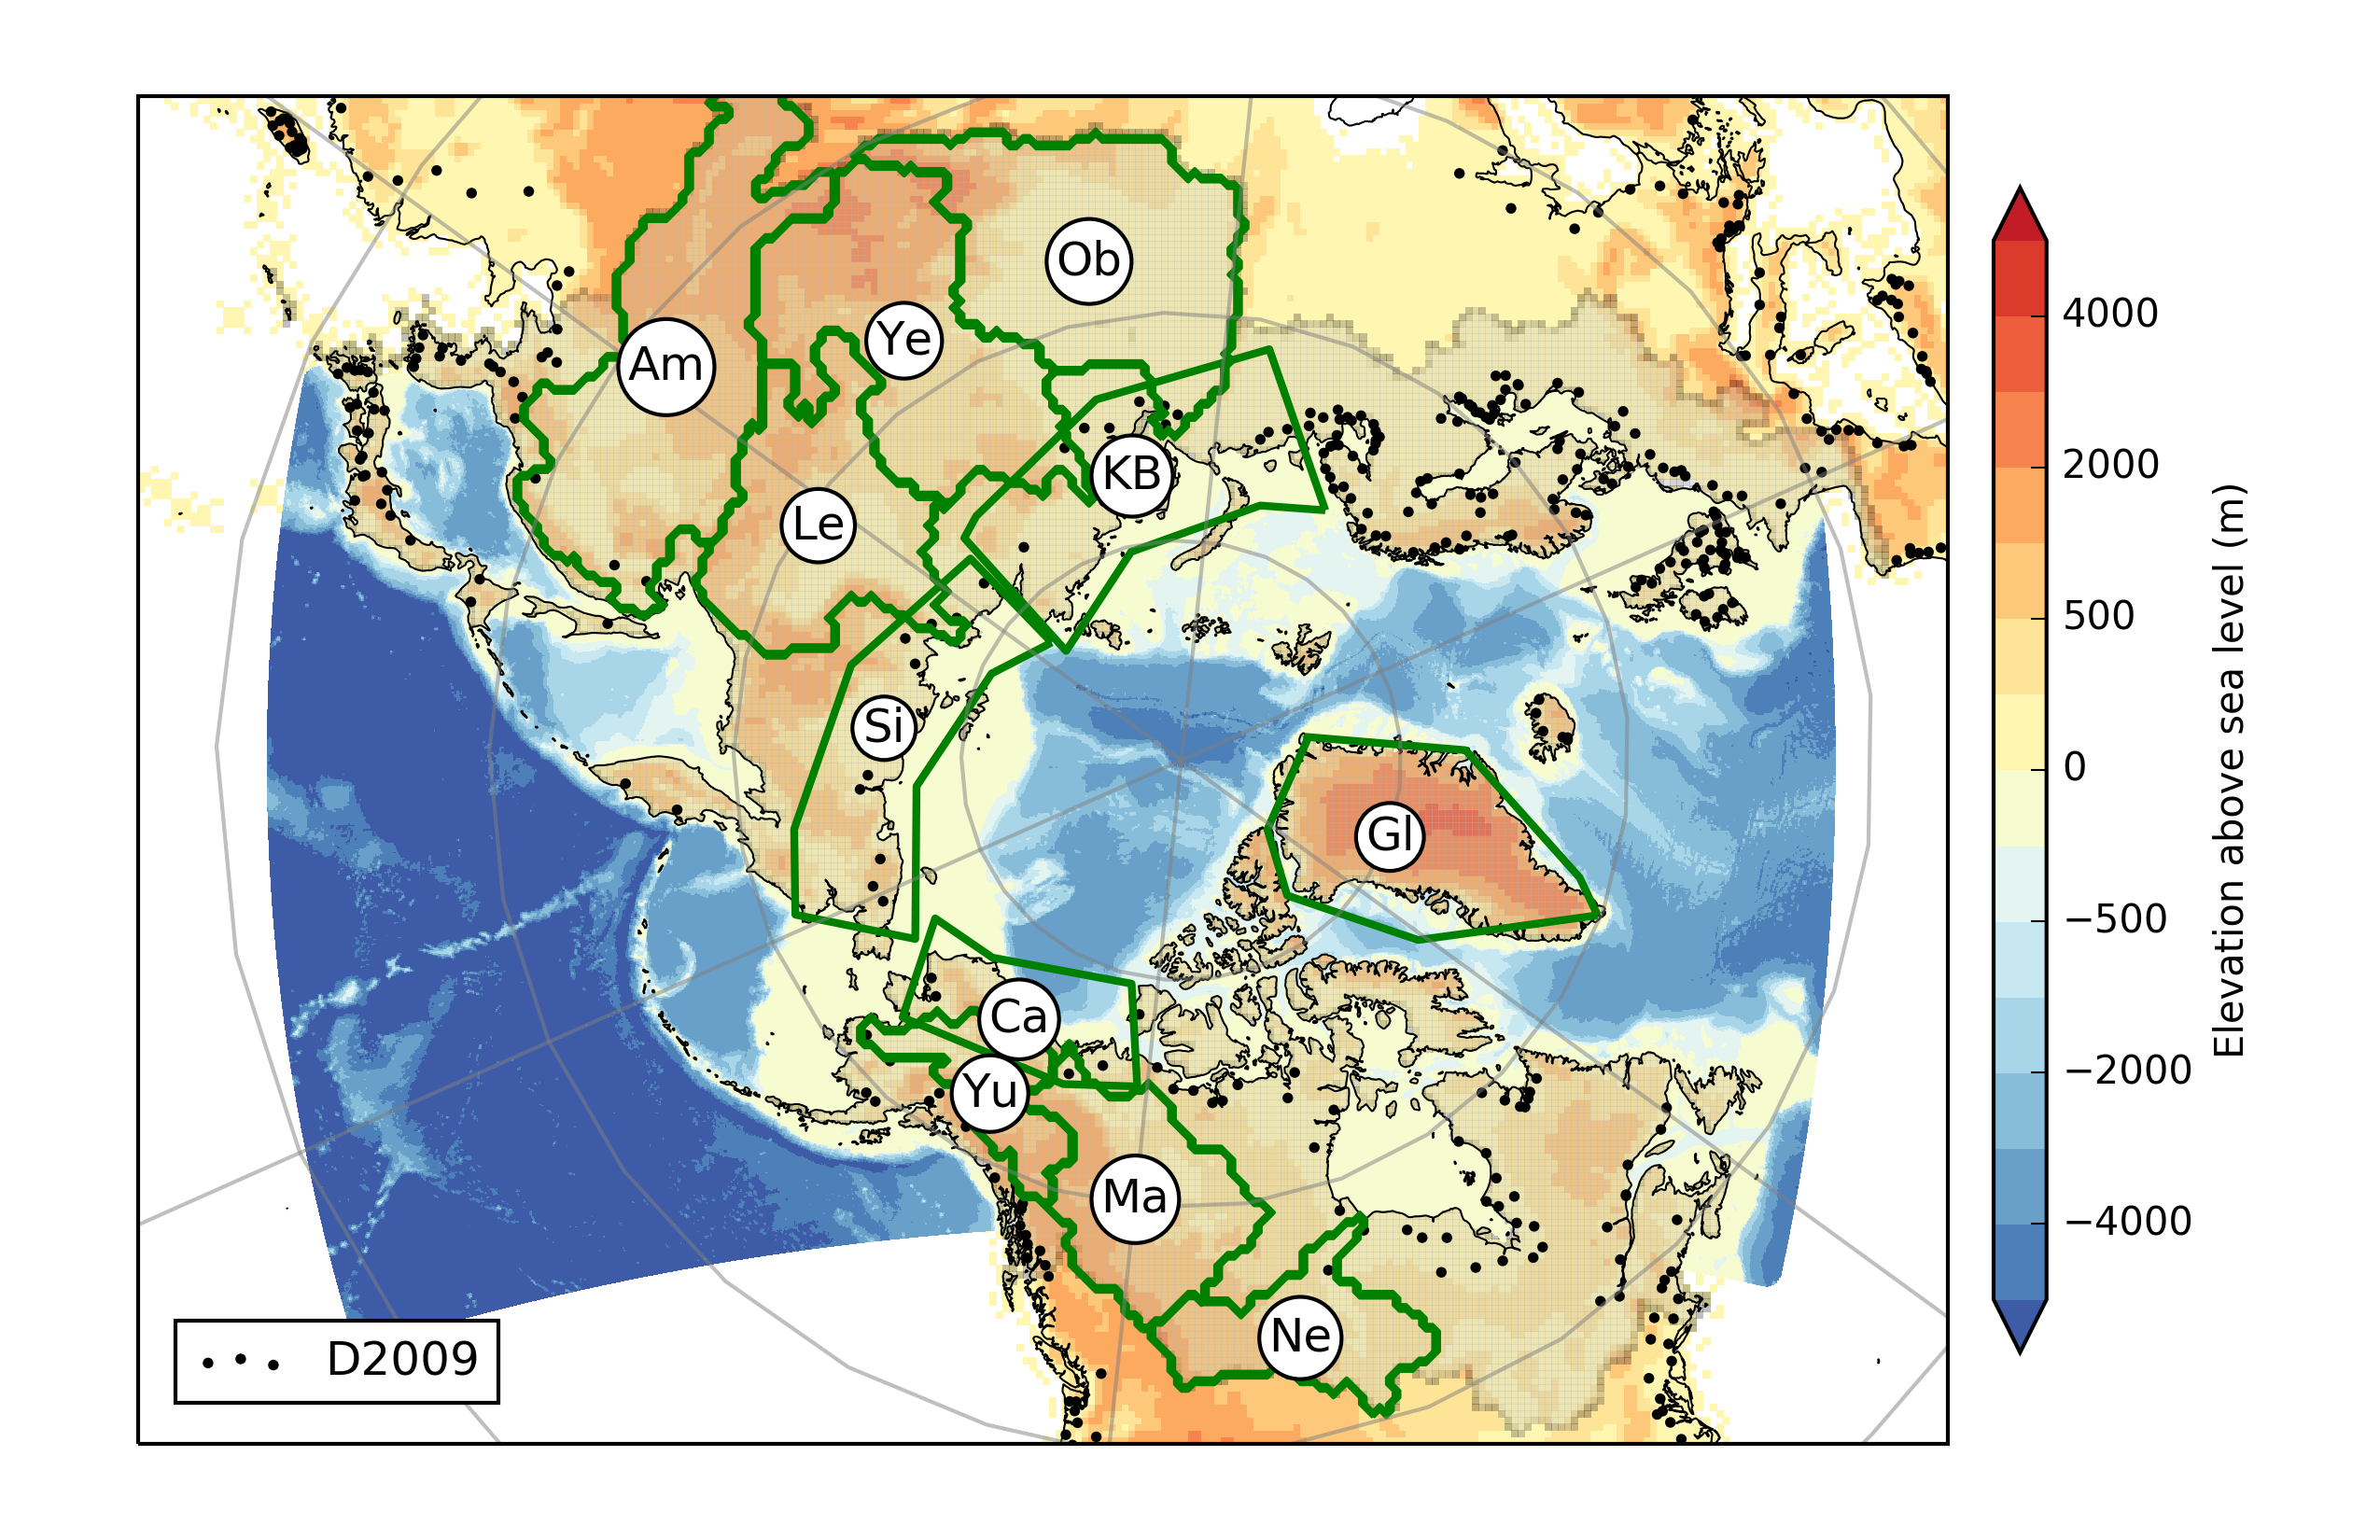
\includegraphics[width=40pc,natwidth=1]{RASM_domain_fig}
\caption{The Regional Arctic System Model domain, showing the 50-km near equal area domain shared by the land, atmosphere, and streamflow routing components (outer rectangle), and the 1/12-degree ocean sea ice domain (blue shading).
The RVIC drainage area is highlighted with gray shading.
The 7 largest river basins in the RASM domain are outlined in green: Amur (Am), Ob' (Ob), Yenisey (Ye), Lena (Le), Mackenzie (Ma), Nelson (Ne), and Yukon (Yu).
The coastal streamflow flux masks used in Section \ref{sec:results} are outlined in green: Canadian Coast (Ca), Siberian Coast (Si), Kara and Barents Coast (KB), and Greenland (Gl). The location of the streamflow observations from $D2009$ are shown with black circles.}
\label{fig:rasm_domain}
\end{figure}

\clearpage
\begin{figure}
\noindent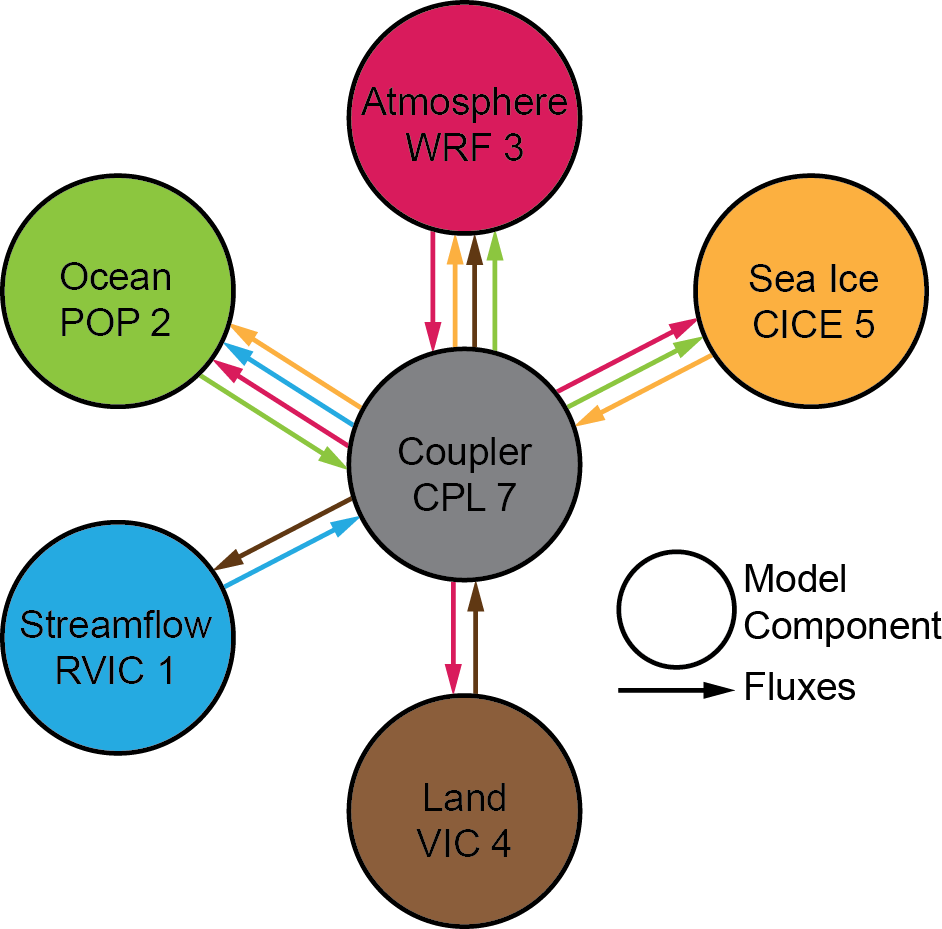
\includegraphics[width=40pc,natwidth=1]{RASM_coupling_schematic}
\caption{Coupling schematic for the Regional Arctic System Model. Circles represent model components (e.g. RVIC) and arrows between circles represent flux and state variables shared between components. The colors of the arrows reflect the source of the fluxes and state variables.}
\label{fig:rasm_coupling_schematic}
\end{figure}

\clearpage
\begin{figure}
\noindent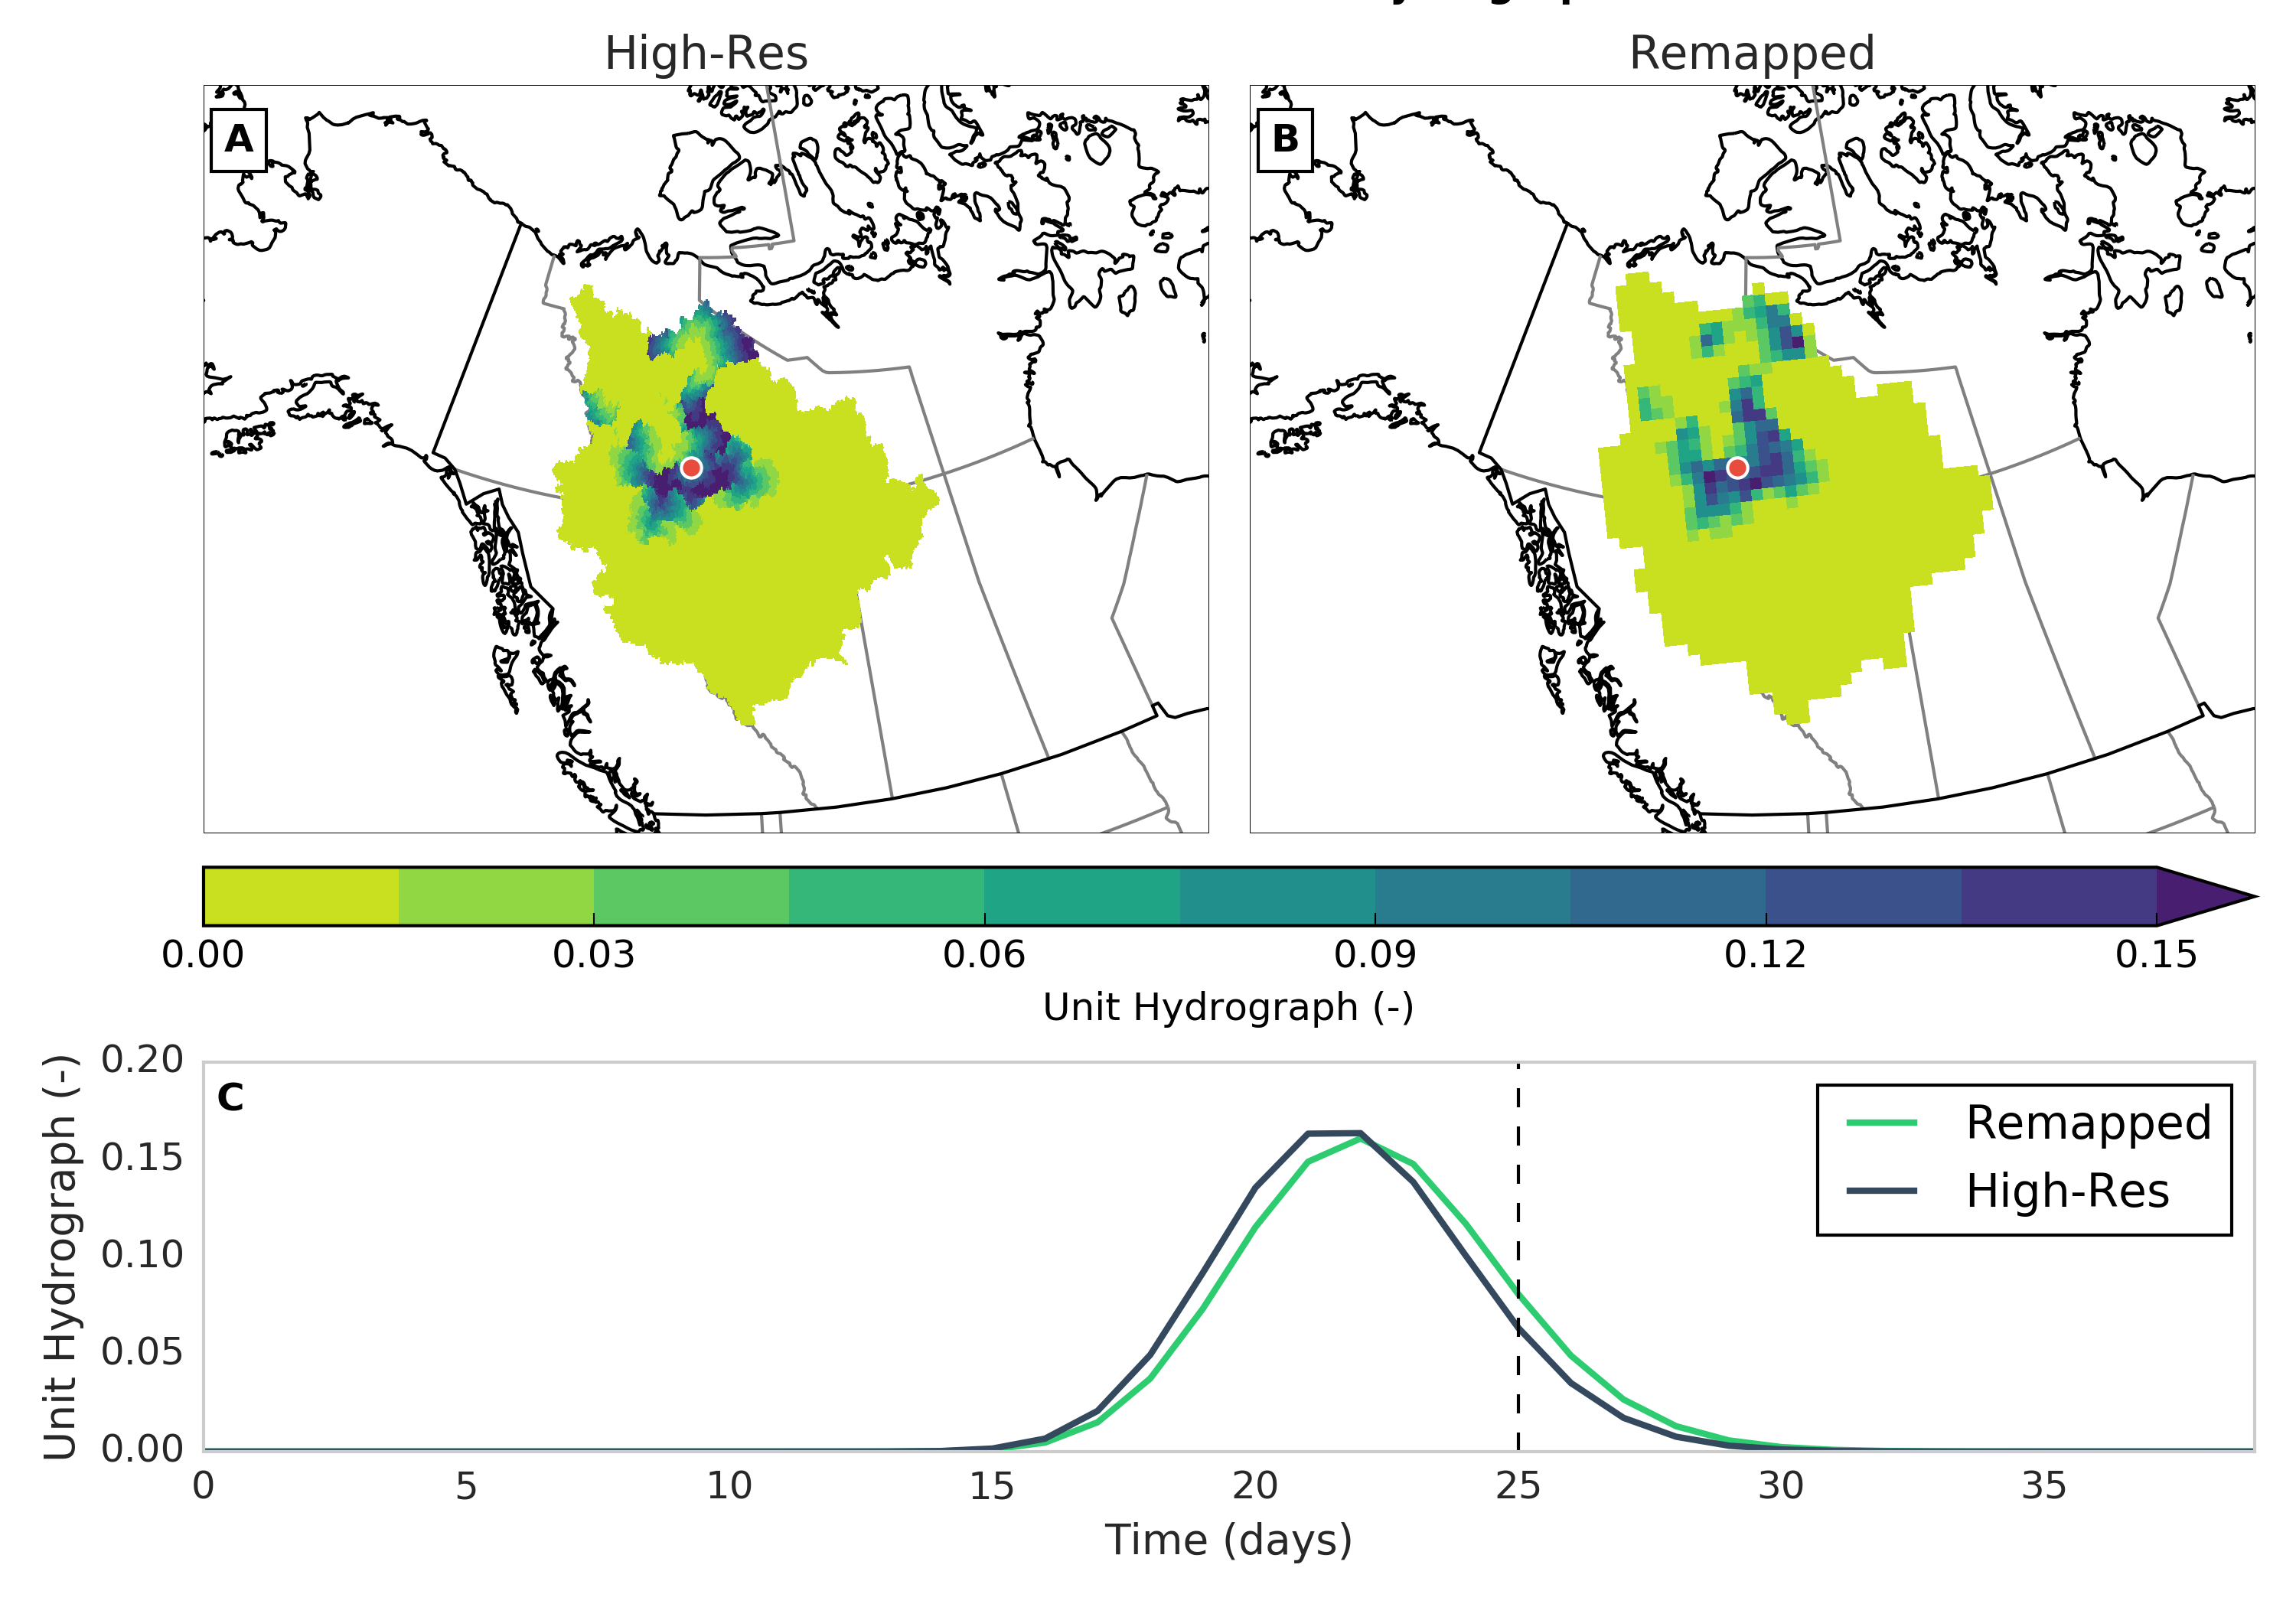
\includegraphics[width=40pc,natwidth=1]{uh_remap_schematic}
\caption{Top: High-resolution (A) and remapped (B) IRFs for the Mackenzie River upstream of the Arctic Red River observation location for timestep 25.
Bottom: IRFs from the high-resolution (blue) and remapped (green) grids at the example point (61.62$^\circ$N, 121.16$^\circ$W) shown in A and B.
The offset between the two IRFs shown in C is the result of the spatial averaging during the remapping.}
\label{fig:uh_remap_schematic}
\end{figure}

\clearpage
\begin{figure}
\noindent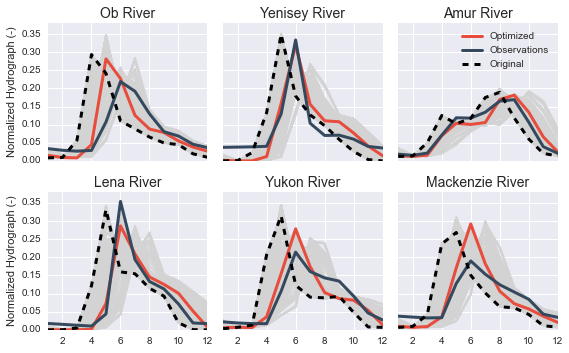
\includegraphics[width=40pc,natwidth=1]{calibration_hydrographs}
\caption{Normalized annual hydrographs for largest six river basins in the RASM domain.
Each trace (grey) represents an individual calibration ensemble member.
The observed (normalized) hydrograph for each basin is shown in blue and the hydrograph using the ``Original'' (``Fast'') parameters is shown with the dashed black line.}
\label{fig:calibration_hydrographs}
\end{figure}

\clearpage
\begin{figure}
\noindent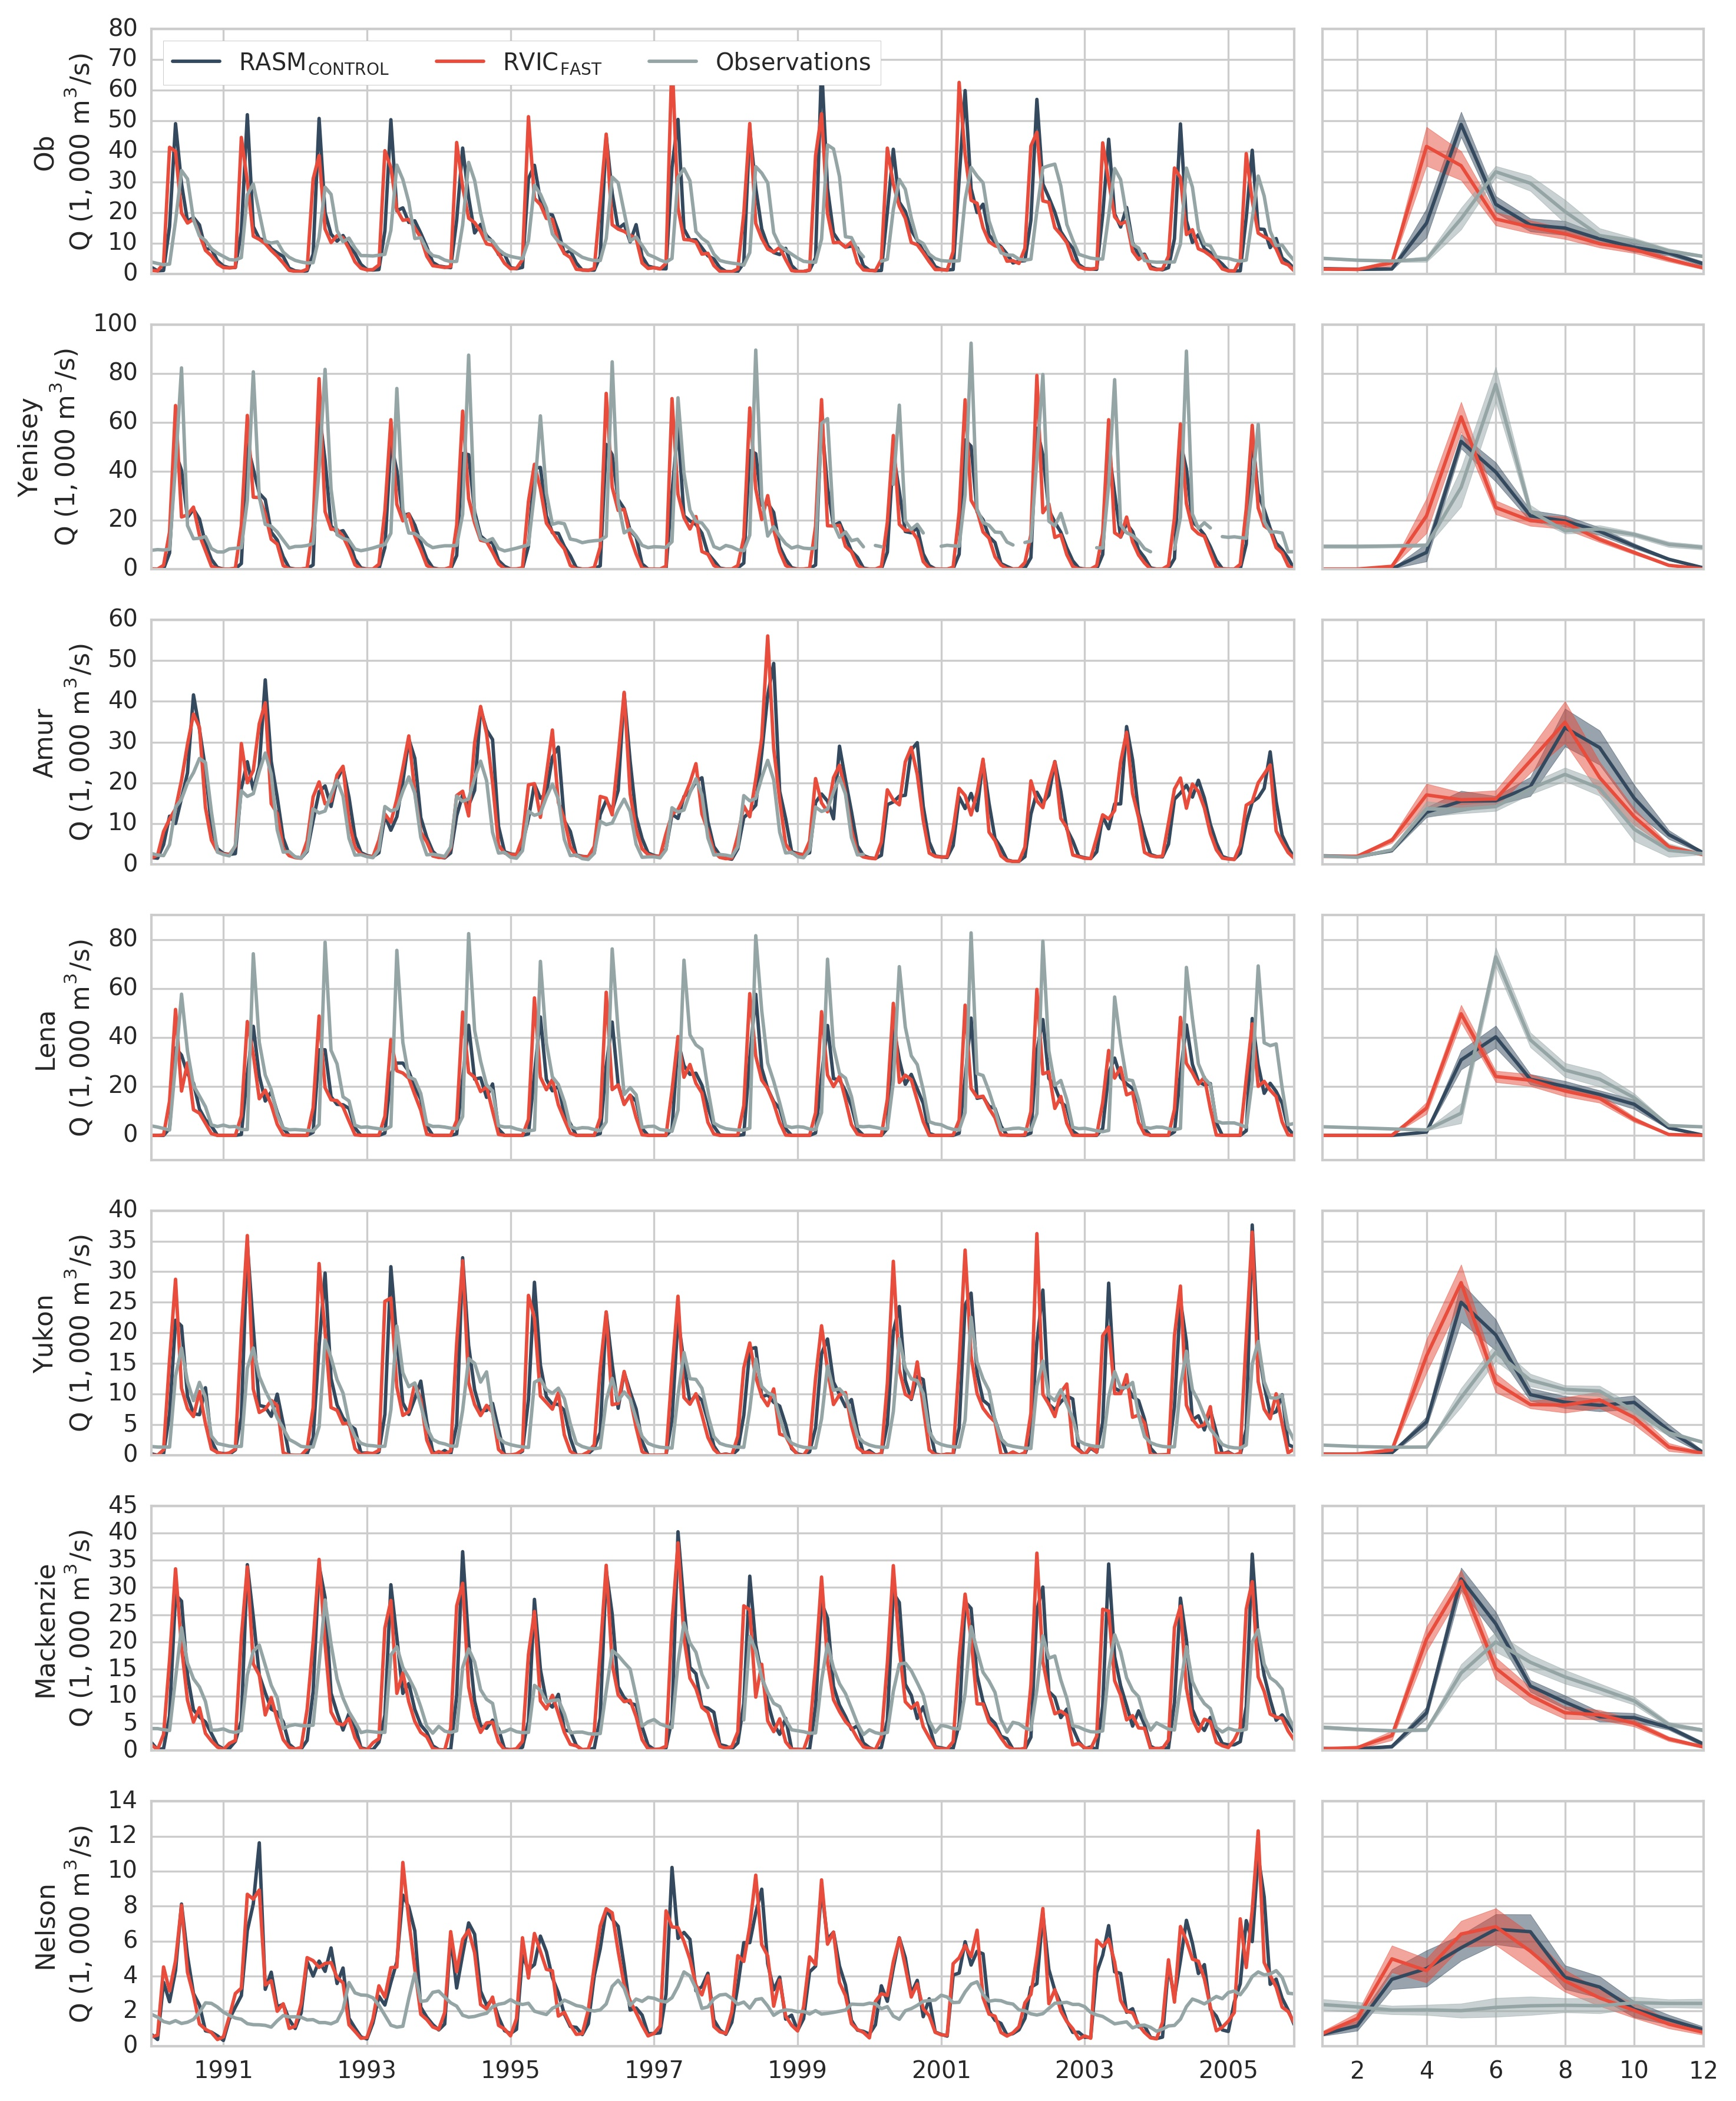
\includegraphics[width=35pc,natwidth=1]{R1010RBRbaaa01a_rvicfast_hydrographs}
\caption{Streamflow hydrographs from $RASM_{CONTROL}$ (blue) and $RVIC_{FAST}$ (red) for the largest seven river basins compared to values from $D2009$ (gray).
The left column includes the monthly streamflow timeseries and the right column includes the monthly mean annual hydrograph where the standard deviation of the interannual variability is represented by the shading.}
\label{fig:hydrographs}
\end{figure}

\clearpage
\begin{figure}
\noindent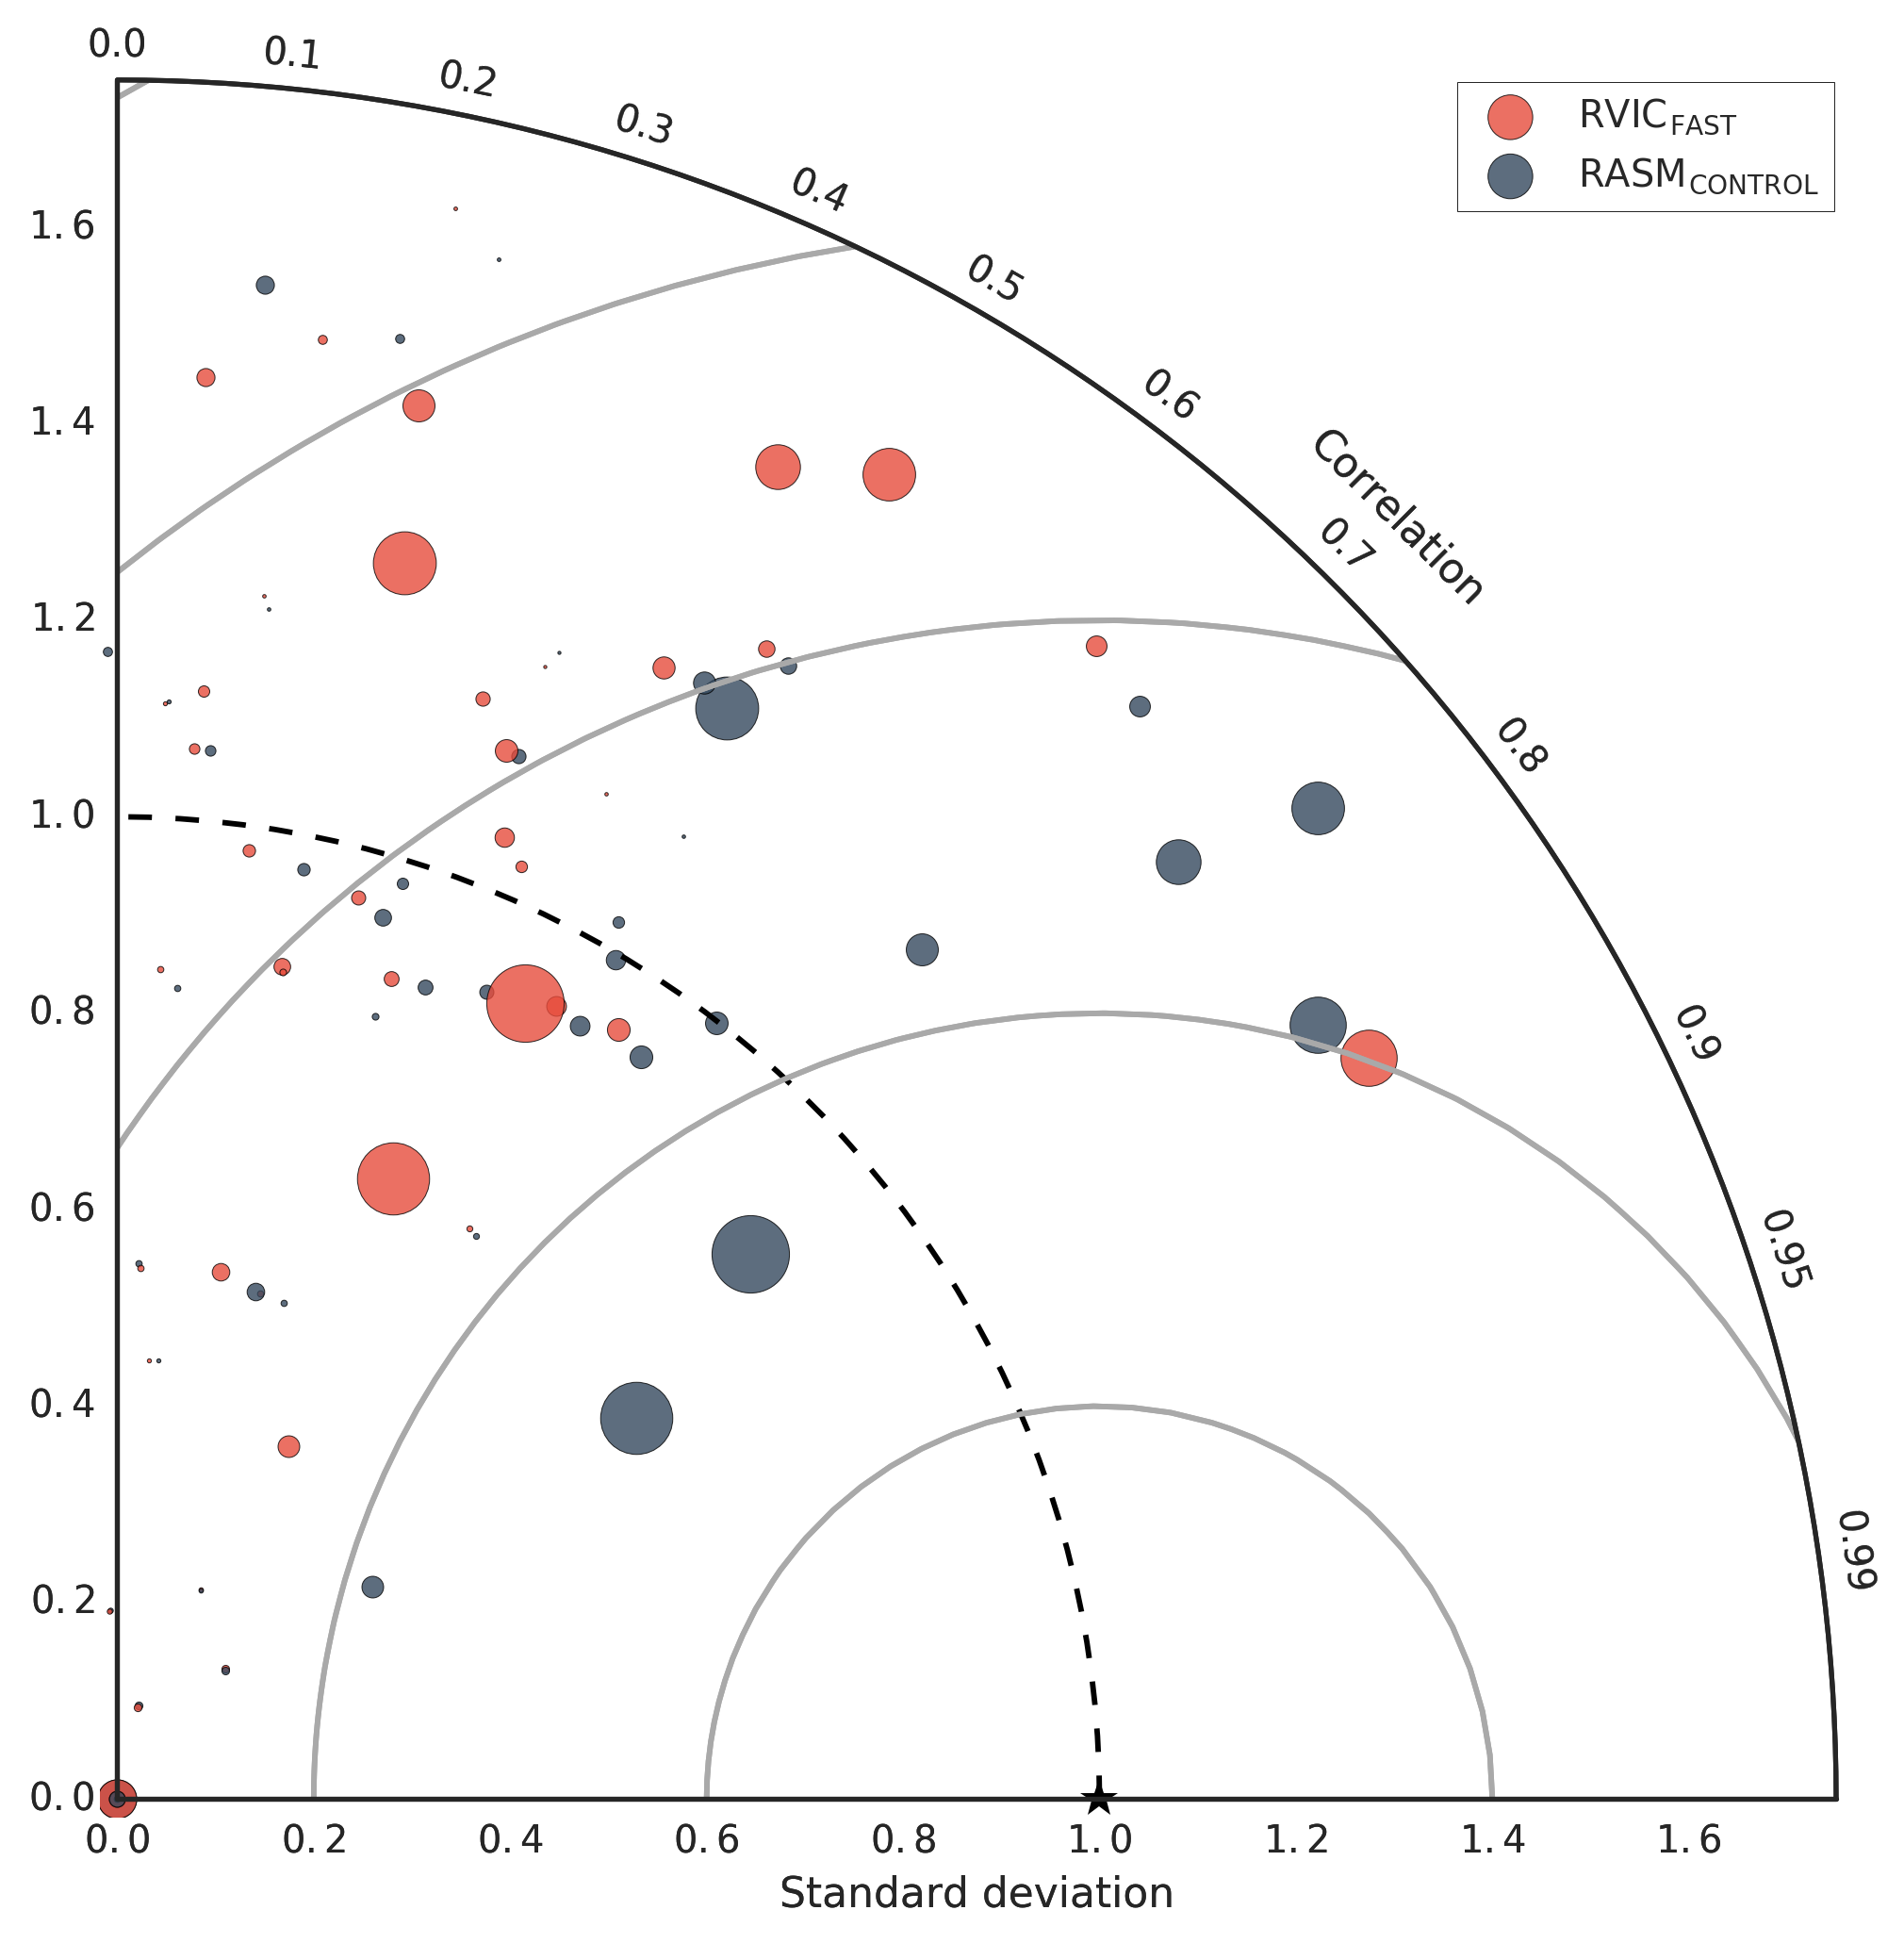
\includegraphics[width=40pc,natwidth=1]{R1010RBRbaaa01a_rvicfast_taylordiag}
\caption{Taylor Diagram showing performance of the RVIC model $RASM_{CONTROL}$ (blue) and $RVIC_{FAST}$ (red) for 51 of the largest rivers in the RASM domain.}
\label{fig:taylor}
\end{figure}

\clearpage
\begin{figure}
\noindent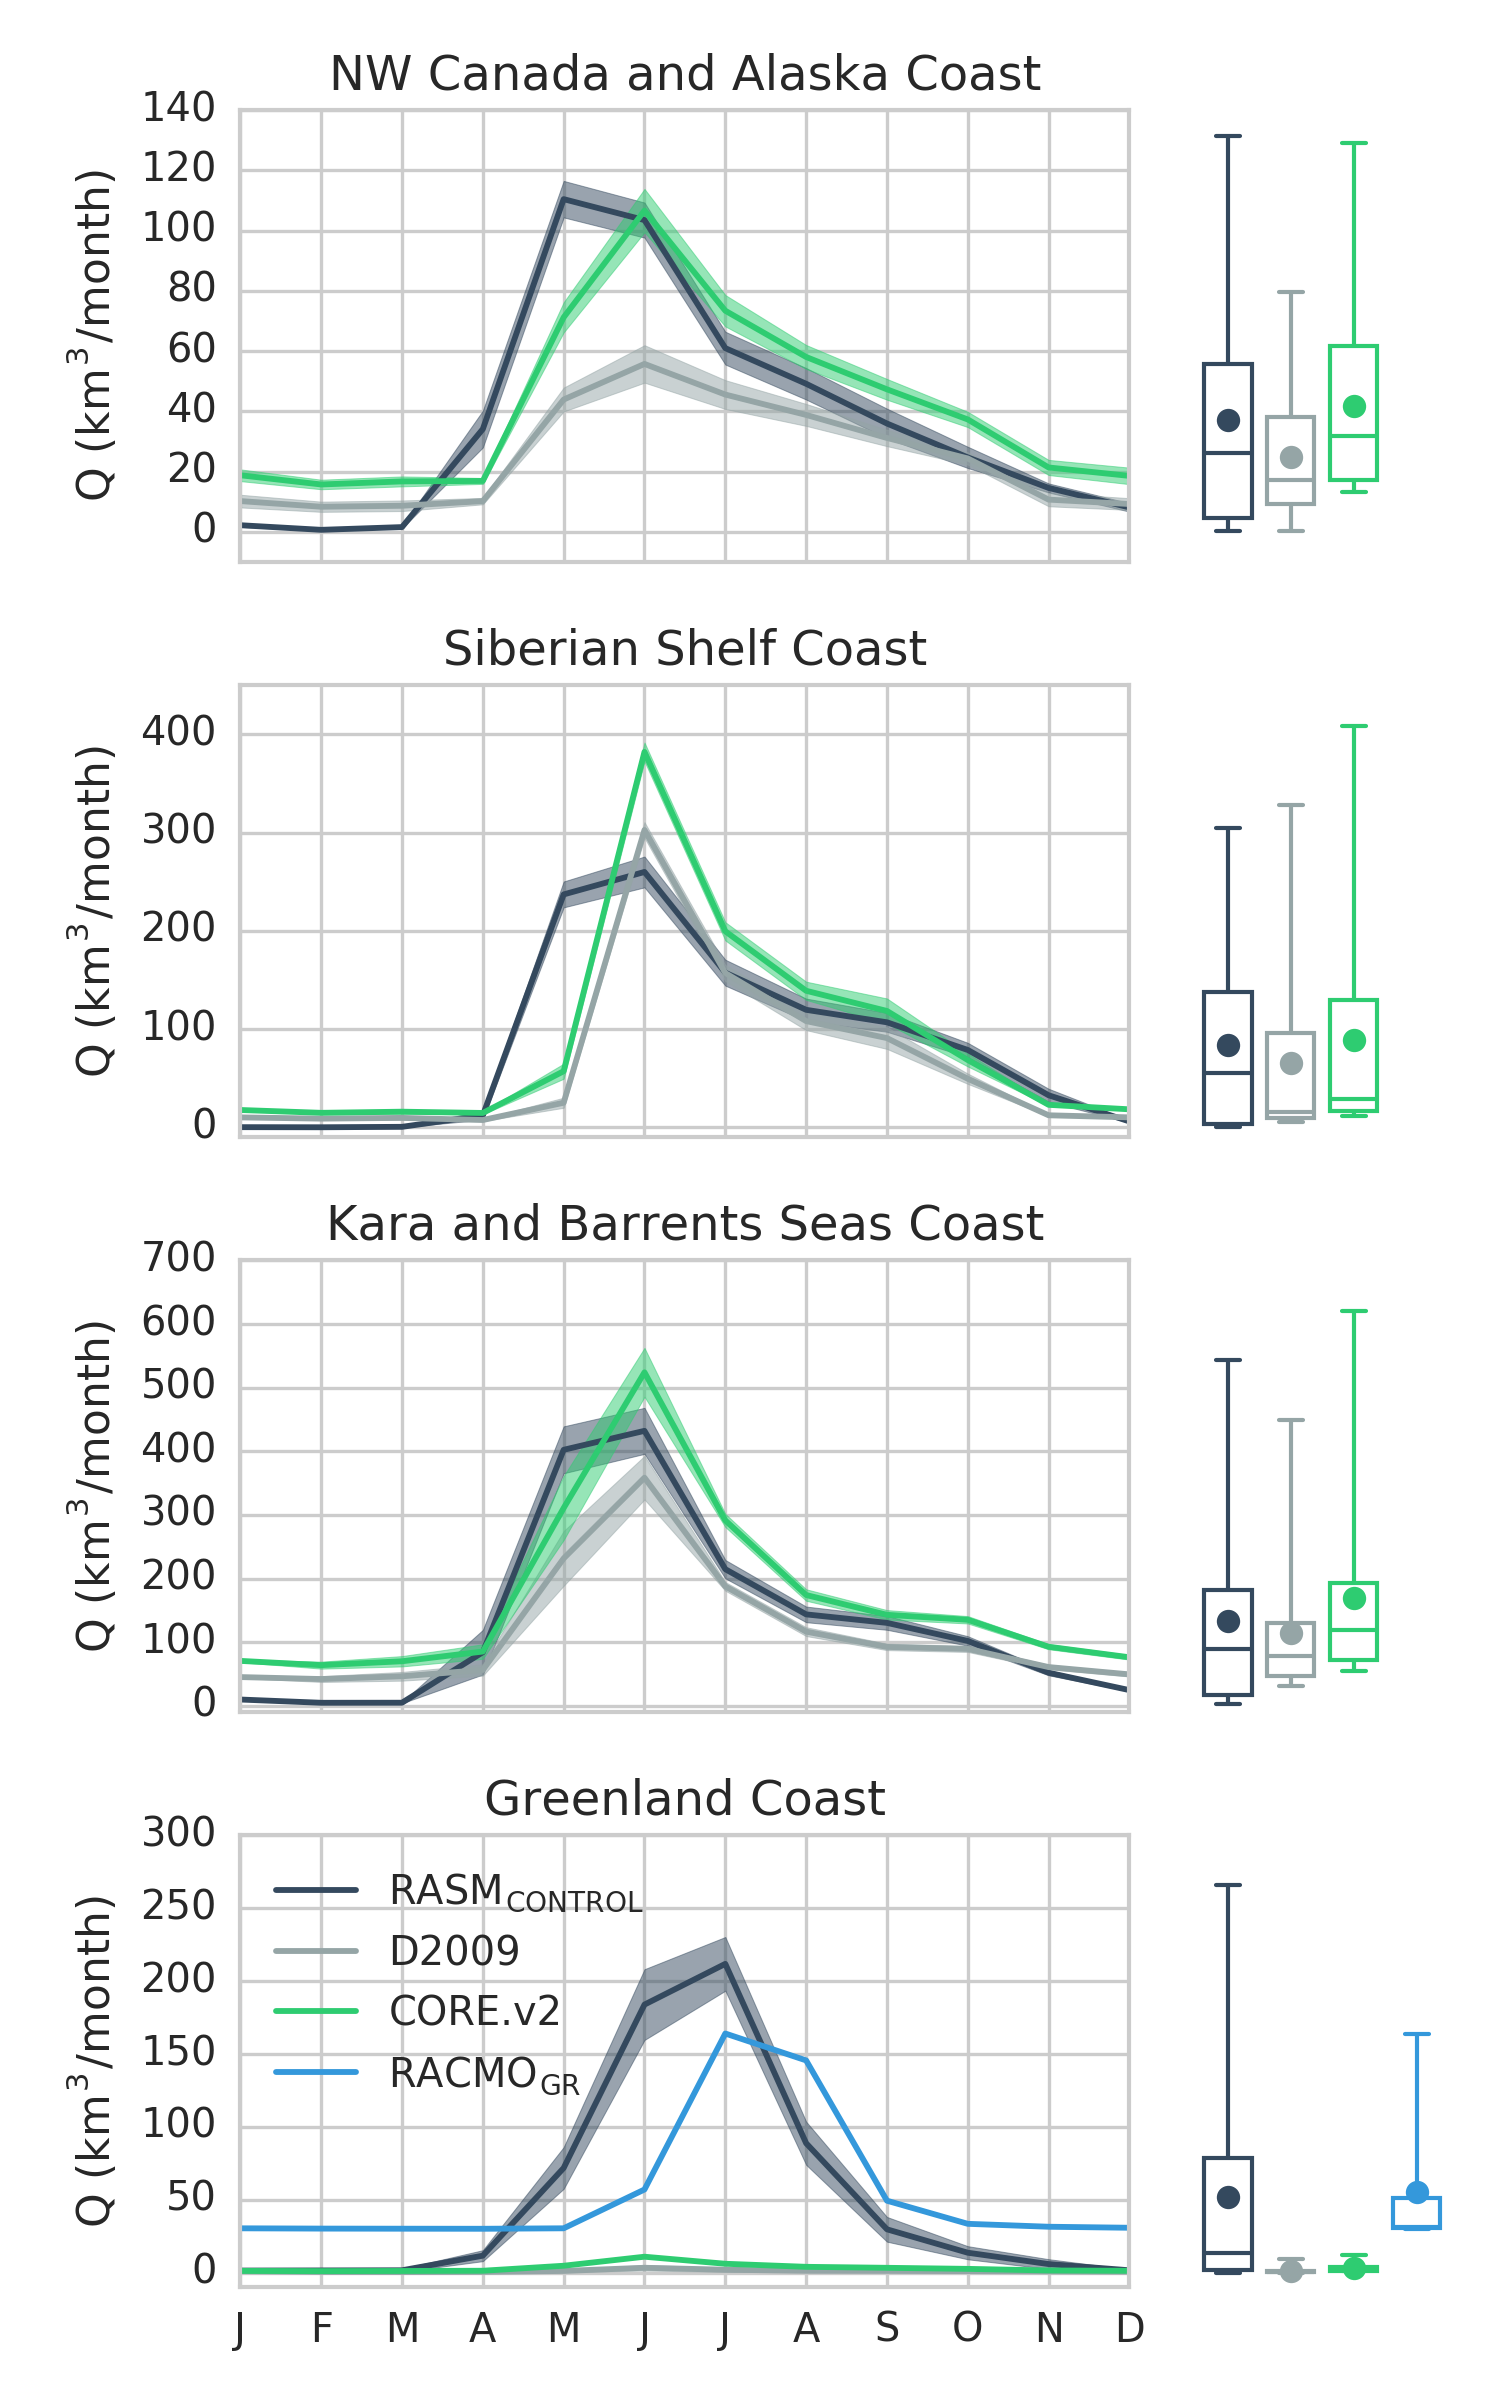
\includegraphics[width=20pc,natwidth=1]{coastal_hydrographs}
\caption{Annual cycle coastal streamflow fluxes for the four masks shown in Figure \ref{fig:rasm_domain} comparing $RASM_{CONTROL}$ (dark blue), $D2009$ (gray), $CORE.v2$ (green), and $Bamber$ (light blue, Greenland only). Solid lines represent the 1991-1999 mean and the shading denotes the interannual variability (not available from $RACMO_{GR}$).}
\label{fig:coastal_hydrographs}
\end{figure}

\clearpage
\begin{figure}
\noindent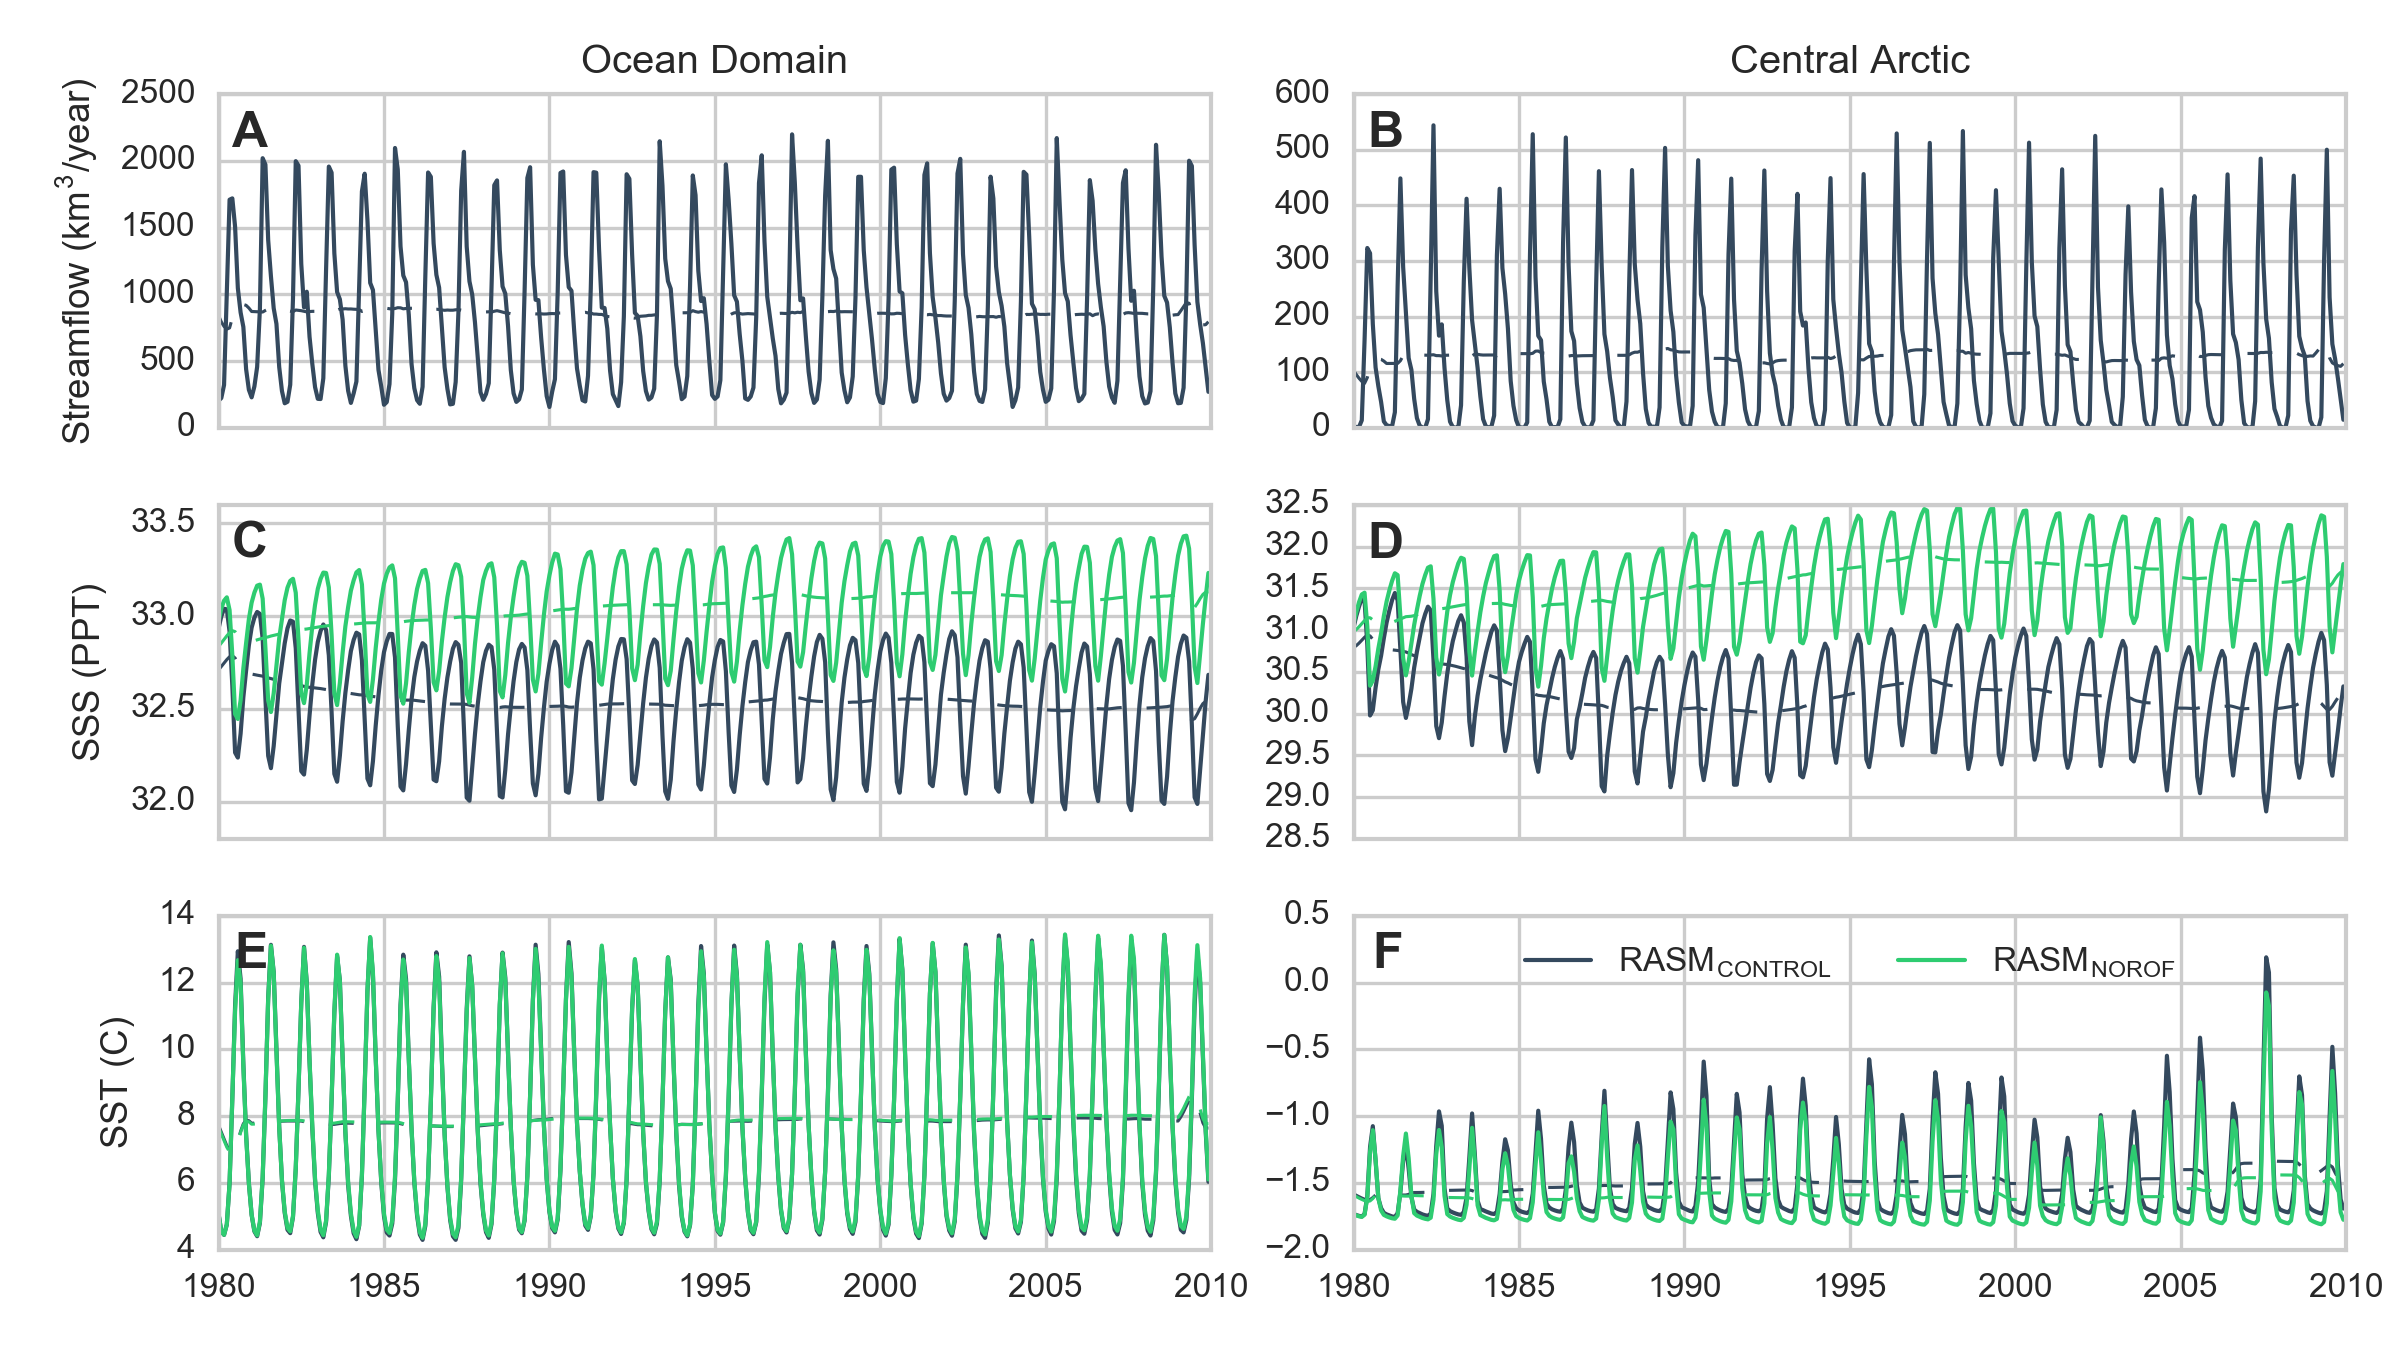
\includegraphics[width=40pc,natwidth=1]{ocean_combine_ts}
\caption{Monthly time series (1980-2009) of domain-wide (left) and central arctic (right) streamflow (top), mean SSS (middle), and SST (bottom) for the $RASM_{CONTROL}$ (blue) and $RASM_{NOROF}$ (green). The dashed lines show a 12-month running mean.}
\label{fig:ocean_timeseries}
\end{figure}

\clearpage
\begin{figure}
\noindent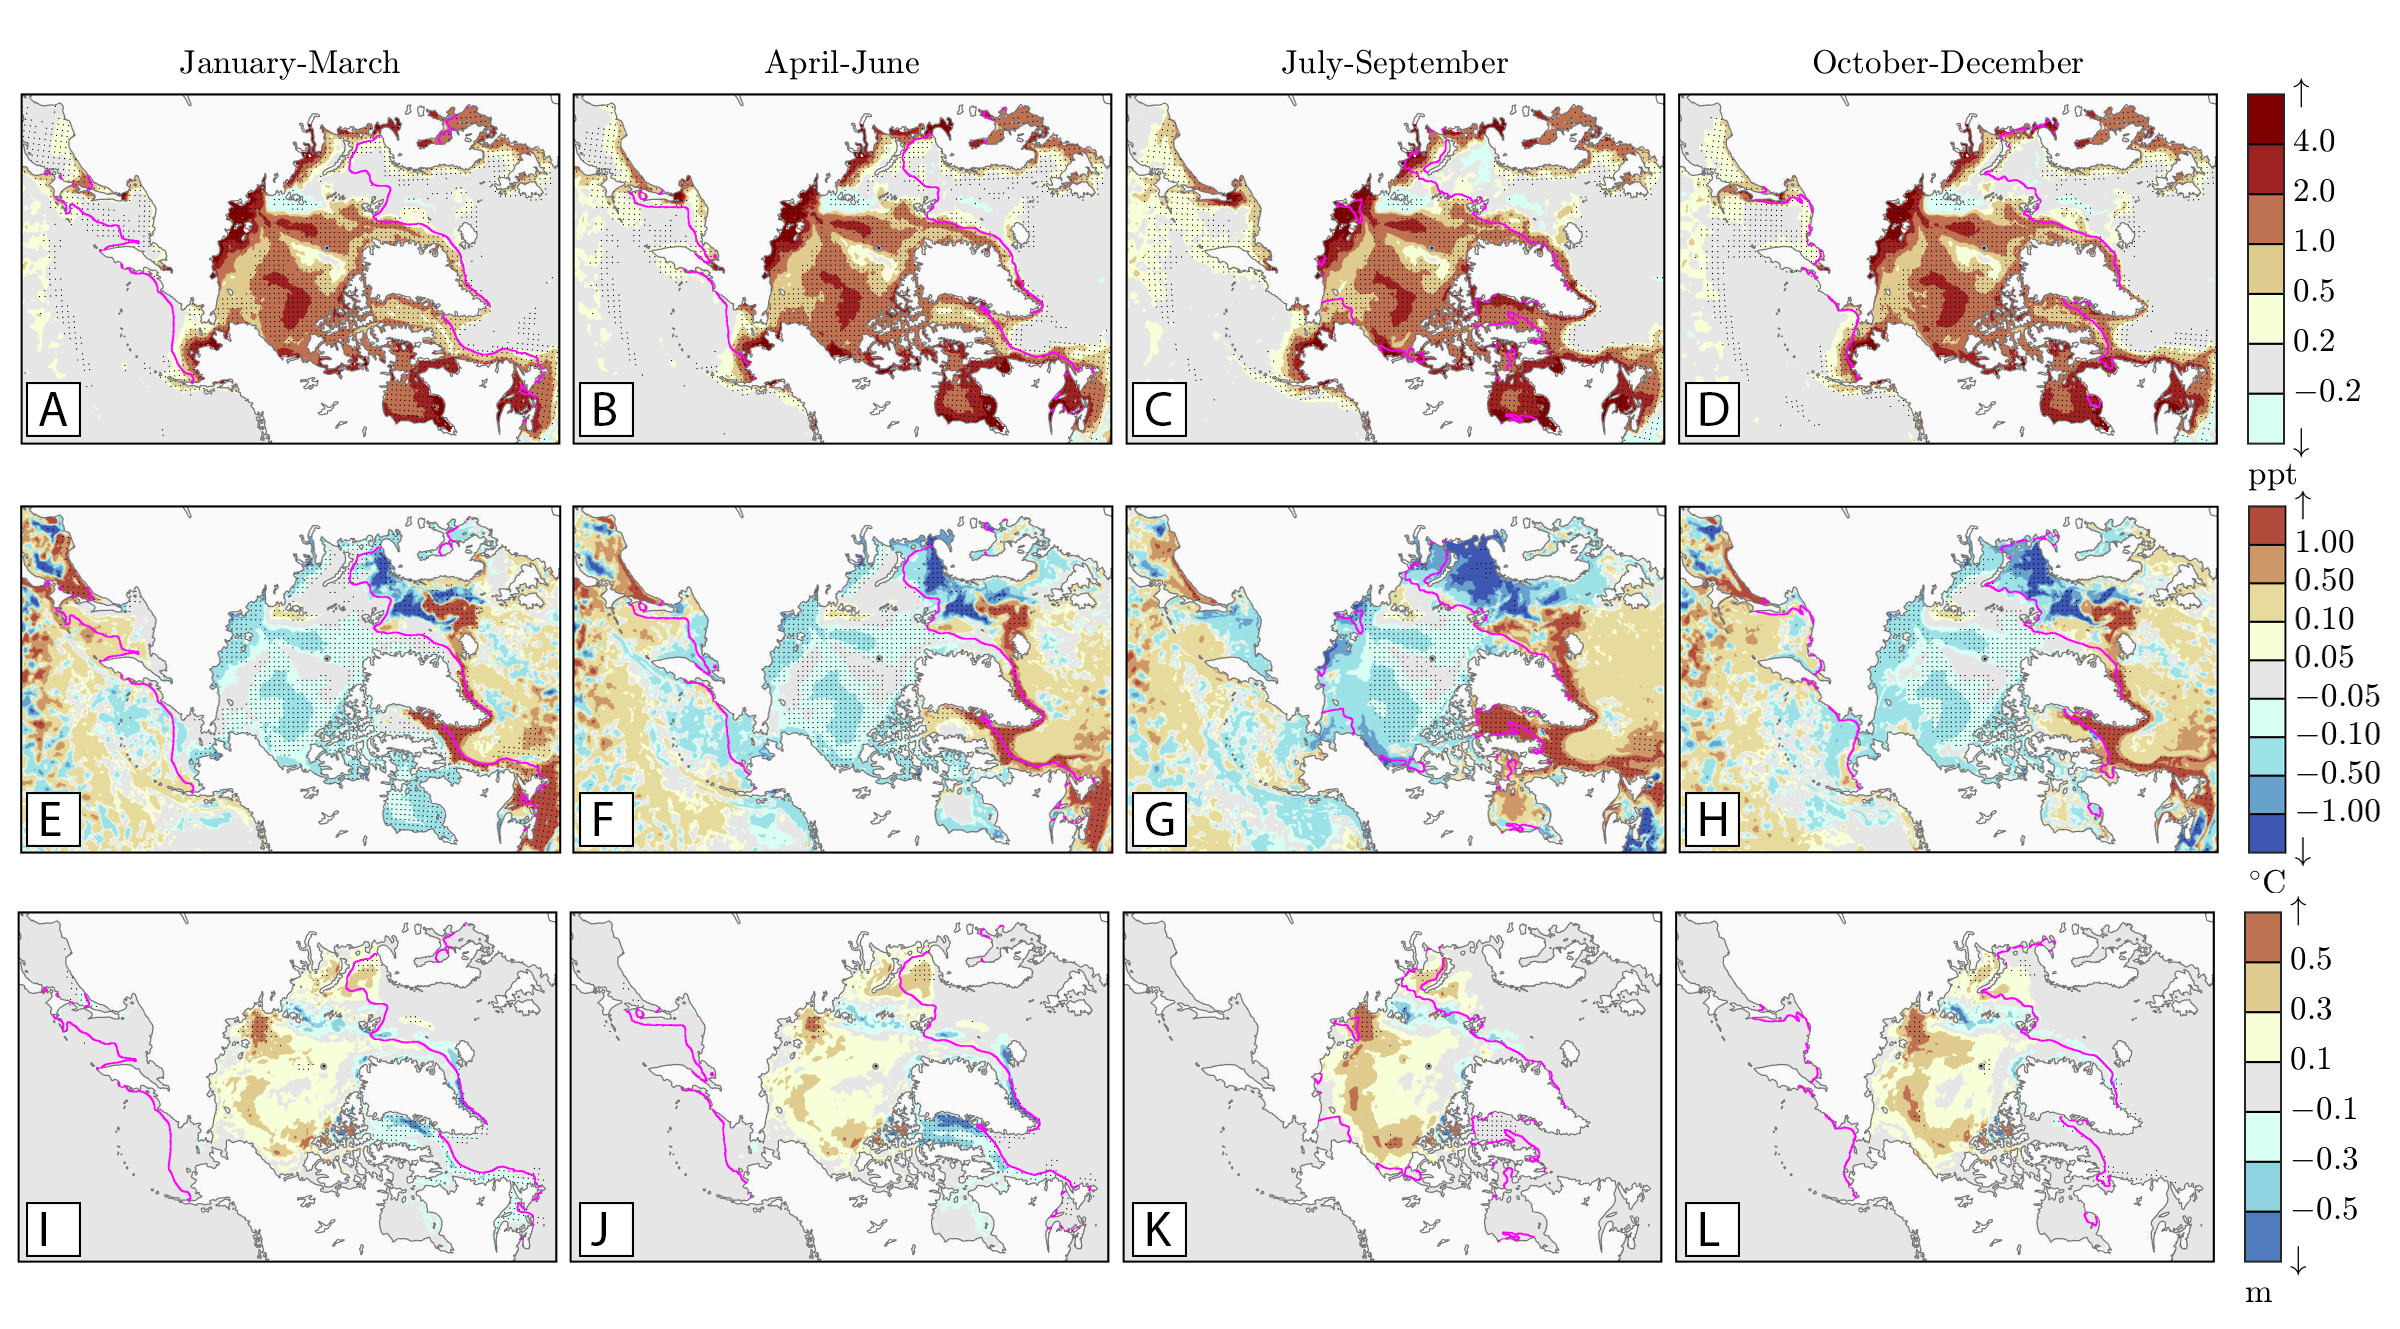
\includegraphics[width=40pc,natwidth=1]{ocean_combine}
\caption{Seasonal difference ($RASM_{NOROF}$ - $RASM_{CONTROL}$) in mean sea surface salinity (top), sea surface temperature (middle), and sea ice height (bottom) (2000-2009). Stippling denotes differences that are statistically significant at the 95 percent confidence interval.}
\label{fig:ocean_maps}
\end{figure}

% Tables
\clearpage

\begin{table}
  \caption{RVIC model performance statistics for the seven rivers shown in Figure \ref{fig:rasm_domain}.}
  \centering
  \label{table:rivers}
  \resizebox{\textwidth}{!}{%
  \begin{tabular}{|l|c|c|c|c|c|c|}
  {} & \multicolumn{1}{c}{Bias (\%)} & \multicolumn{2}{c}{Overlap (-)}  &  \multicolumn{2}{c}{RMSE (100 $m^3/s$)} \\
  River                   & $RASM_{CONTROL}$ & $RVIC_{FAST}$ & $RASM_{CONTROL}$ & $RVIC_{FAST}$ & $RASM_{CONTROL}$ \\
  Ob' at Salekhard         &            -3.9  &          0.65 &             0.73 &      148.7    &         120.9    \\
  Yenisey at Igarka       &           -25.8  &          0.64 &             0.75 &      201.1    &         137.9    \\
  Amur at Komsomolsk      &            26.9  &          0.93 &             0.90 &       67.1    &          68.3    \\
  Lena at Kusur           &           -28.0  &          0.64 &             0.80 &      207.3    &         137.1    \\
  Yukon at Pilot          &            13.2  &          0.66 &             0.79 &       73.6    &          50.9    \\
  Mackenzie at Arctic Red &            -4.0  &          0.67 &             0.75 &       82.2    &          62.2    \\
  Nelson at Bladder       &            61.3  &          0.70 &             0.71 &       29.2    &          28.8    \\
  \end{tabular}
}
\end{table}

\end{document}

%%%%%%%%%%%%%%%%%%%%%%%%%%%%%%%%%%%%%%%%%%%%%%%%%%%%%%%%%%%%%%%

More Information and Advice:

%% ------------------------------------------------------------------------ %%
%
%  SECTION HEADS
%
%% ------------------------------------------------------------------------ %%

% Capitalize the first letter of each word (except for
% prepositions, conjunctions, and articles that are
% three or fewer letters).

% AGU follows standard outline style; therefore, there cannot be a section 1 without
% a section 2, or a section 2.3.1 without a section 2.3.2.
% Please make sure your section numbers are balanced.
% ---------------
% Level 1 head
%
% Use the \section{} command to identify level 1 heads;
% type the appropriate head wording between the curly
% brackets, as shown below.
%
%An example:
%\section{Level 1 Head: Introduction}
%
% ---------------
% Level 2 head
%
% Use the \subsection{} command to identify level 2 heads.
%An example:
%\subsection{Level 2 Head}
%
% ---------------
% Level 3 head
%
% Use the \subsubsection{} command to identify level 3 heads
%An example:
%\subsubsection{Level 3 Head}
%
%---------------
% Level 4 head
%
% Use the \subsubsubsection{} command to identify level 3 heads
% An example:
%\subsubsubsection{Level 4 Head} An example.
%
%% ------------------------------------------------------------------------ %%
%
%  IN-TEXT LISTS
%
%% ------------------------------------------------------------------------ %%
%
% Do not use bulleted lists; enumerated lists are okay.
% \begin{enumerate}
% \item
% \item
% \item
% \end{enumerate}
%
%% ------------------------------------------------------------------------ %%
%
%  EQUATIONS
%
%% ------------------------------------------------------------------------ %%

% Single-line equations are centered.
% Equation arrays will appear left-aligned.

Math coded inside display math mode \[ ...\]
 will not be numbered, e.g.,:
 \[ x^2=y^2 + z^2\]

 Math coded inside \begin{equation} and \end{equation} will
 be automatically numbered, e.g.,:
 \begin{equation}
 x^2=y^2 + z^2
 \end{equation}

% IF YOU HAVE MULTI-LINE EQUATIONS, PLEASE
% BREAK THE EQUATIONS INTO TWO OR MORE LINES
% OF SINGLE COLUMN WIDTH (20 pc, 8.3 cm)
% using double backslashes (\\).

% To create multiline equations, use the
% \begin{eqnarray} and \end{eqnarray} environment
% as demonstrated below.
\begin{eqnarray}
  x_{1} & = & (x - x_{0}) \cos \Theta \nonumber \\
        && + (y - y_{0}) \sin \Theta  \nonumber \\
  y_{1} & = & -(x - x_{0}) \sin \Theta \nonumber \\
        && + (y - y_{0}) \cos \Theta.
\end{eqnarray}

%If you don't want an equation number, use the star form:
%\begin{eqnarray*}...\end{eqnarray*}

% Break each line at a sign of operation
% (+, -, etc.) if possible, with the sign of operation
% on the new line.

% Indent second and subsequent lines to align with
% the first character following the equal sign on the
% first line.

% Use an \hspace{} command to insert horizontal space
% into your equation if necessary. Place an appropriate
% unit of measure between the curly braces, e.g.
% \hspace{1in}; you may have to experiment to achieve
% the correct amount of space.


%% ------------------------------------------------------------------------ %%
%
%  EQUATION NUMBERING: COUNTER
%
%% ------------------------------------------------------------------------ %%

% You may change equation numbering by resetting
% the equation counter or by explicitly numbering
% an equation.

% To explicitly number an equation, type \eqnum{}
% (with the desired number between the brackets)
% after the \begin{equation} or \begin{eqnarray}
% command.  The \eqnum{} command will affect only
% the equation it appears with; LaTeX will number
% any equations appearing later in the manuscript
% according to the equation counter.
%

% If you have a multiline equation that needs only
% one equation number, use a \nonumber command in
% front of the double backslashes (\\) as shown in
% the multiline equation above.

%% ------------------------------------------------------------------------ %%
%
%  SIDEWAYS FIGURE AND TABLE EXAMPLES
%
%% ------------------------------------------------------------------------ %%
%
% For tables and figures, add \usepackage{rotating} to the paper and add the rotating.sty file to the folder.
% AGU prefers the use of {sidewaystable} over {landscapetable} as it causes fewer problems.
%
% \begin{sidewaysfigure}
% \includegraphics[width=20pc]{samplefigure.eps}
% \caption{caption here}
% \label{label_here}
% \end{sidewaysfigure}
%
%
%
% \begin{sidewaystable}
% \caption{}
% \begin{tabular}
% Table layout here.
% \end{tabular}
% \end{sidewaystable}
%
%
